\documentclass{article}

\usepackage{kyblab}
\usepackage{tabstackengine}
\stackMath
\newcommand{\bm}[1]{\boldsymbol{\mathrm{#1}}}
\setlength\parindent{0pt}
\usepackage{marvosym}
\usepackage{color}
\usepackage{float}

\title{%
    Helicopter control using linear control theory \\ \medskip
    \large{Helicopter lab for TTK4115 at NTNU}}

\author{
Alexander Johansen - 759059\\ 
Lars C. M. van der Lee - 768644\\
Åshild Lien - 768635\\
Group 43}


\date{October 2017}

\begin{document}

\maketitle

\newpage

\tableofcontents

\newpage
%\section*{Abstract}

This report is 

% miniature report % We drop this

\section{Introduction}
This lab assignment aims to use linear control theory to allow the control of a helicopter using a joystick. Trying to control the helicopter, without a regulator to stabilize the system, is nearly impossible. The helicopter becomes hard to control, and will crash if the user makes a small mistake.

\begin{figure}[htb]
	\centering
	\includegraphics[width=0.9\linewidth]{images/helicopter.pdf}
    \caption{Helicopter setup, \cite{HeliLabAssignment}}
    \label{fig:setup}
\end{figure}


Figure \ref{fig:setup} shows the helicopter setup used in the lab. The 2 propellers are balanced with a counterweight on the other side of the center joint. These are controlled by changing the voltage to each motor. \medskip

To complete the task, we have derived a model for the helicopter system. In the different sub problems of the lab assignment, this model will be used to test different regulators. During the lab, we are testing P, PD and multivariable controllers. In the last part of the lab we will also implement an estimator for the states, and use observability to estimate states that aren't measured. This will be combined with an LQR regulator to control the helicopter. \medskip

This rapport will have two main parts, theory and results. During the theory we will derive all the equations for our model and controllers. The results will showcase the helicopter behaviour, and compare it to other controllers. Here we also discuss why some controllers work better than others.\medskip

Tables with constants and parameters can be found in Appendix \ref{sec:nomenclature}. Appendix \ref{sec:matlab_snippets} contains Matlab code snippets. We used Matlab 2014a in the lab.
\section{Theory}

% This file should include project description and a model of the helicopter
%%%%%%%%%%%%%%%%%%%%%%%%%%%%%%%%%%%%%%%%%%%%%%%%%%%%%%%%%%%%%%%%%%%%%%%%%%%%%%%%%%%%%%%%%%%%

%%%%                                PART 1 PROBLEM 1

%%%%%%%%%%%%%%%%%%%%%%%%%%%%%%%%%%%%%%%%%%%%%%%%%%%%%%%%%%%%%%%%%%%%%%%%%%%%%%%%%%%%%%%%%%%%
\subsection{Part 1: Feed Forward}
\subsubsection{Problem 1}

The relations between motor voltage, and actual force delivered are given by
\begin{subequations} \label{eq:part1_prob1_forces}
    \begin{align}
        F_f &= K_f V_f \\
        F_b &= K_f V_b
    \end{align}
\end{subequations}

where $F_b$ and $F_f$ are propeller forces, $V_b$ and $V_f$ are motor voltages and $K_f$ is the motor force constant. Our regulator will create two outputs, $V_s$ and $V_d$, which relate to the actual motor voltages like this:
\begin{subequations} \label{eq:voltages}
    \begin{align}
        V_s &= V_f + V_b \label{eq:voltages_vs}\\
        V_d &= V_f - V_b \label{eq:voltages_vd}
    \end{align}
\end{subequations}


We start with the momentum equations, derived from Newton's second law, 
\begin{equation} \label{eq:part1_prob1_momentum_general}
    \sum M = J \alpha
\end{equation}

where $M$ is torque, $J$ is  moment of inertia and $\alpha$ is angular acceleration. The moment around the pitch joint, $J_p\ddot{p}$, is affected by four forces. The propeller forces generated by their blades, and their weight. Since our propellers have the same weight, and are mounted on each side of the joint, the weight forces cancel each other out. 
Therefore only the forces generated by the blades affect the moment. Propellers are mounted a distance $l_p$ from the pitch joint, giving us the following expression for moment around the pitch joint:
\begin{equation}
    J_{p} \ddot{p} = l_p F_f - l_p F_p
\end{equation}

Substituting $F_f$ and $F_b$ with $V_d$ given from eqs. (\ref{eq:part1_prob1_forces}) and (\ref{eq:voltages_vd}) gives

\begin{equation}
    J_p \ddot{p} = l_p K_f V_d
\end{equation}

By defining $L_1 = l_p K_f$, we find the equation of motion for pitch to be

\begin{equation} \label{eq:model_pitch}
    J_p \ddot{p} = L_1 V_d
\end{equation}

The moment around the elevation joint is affected by the three gravitational forces from the propellers and the counterweight, and can be described by the equation
\begin{equation}
    J_e \ddot{e} = (F_{g, c} l_{c} - (F_{g, f} + F_{g, b}) l_h) \cos (e) + ((F_f + F_b) l_h) \cos(p)
\end{equation}

where $e$ is the elevation angle. Choosing $L_2 = F_{g, c} l_c - (F_{g, f} + F_{g, b}) l_h$, using eqs. (\ref{eq:part1_prob1_forces}) and (\ref{eq:voltages_vs}) to substitute $F_f$ and $F_b$ and then setting $L_3 = K_f l_h$, we get the second equation of motion on the desired form:

\begin{equation} \label{eq:model_elev}
    J_e \ddot{e} = L_2 \cos (e) + L_3 V_s \cos (p)
\end{equation}

%Momentum equation for elevation gives
%\begin{equation}
%    L_2 = F_{g, c} l_c - (F_{g, g} + F_{g, b}) l_h
%\end{equation}

%\begin{equation}
%    L_3 = K_f l_h
%\end{equation}

Only the propeller forces contribute to moment around the travel joint. The way the assignment defines direction for pitch and travel cause the need of a minus sign on the equation, given by
\begin{equation}
    J_{\lambda} \ddot{\lambda} = -(F_f + F_b) l_h l_p \sin (p) \cos (e)
\end{equation}

where $\lambda$ is the travel angle. Again, we substitute $F_f + F_b = K_f V_s$ and define $L_4 = -K_f l_h$ and the equation of motion becomes
\begin{equation}
    J_{\lambda} \ddot{\lambda} = L_4 V_s \sin (p) \cos (e)
\end{equation}

Below are all the equations that make up our model of the helicopter, with their constants:

\begin{subequations}\label{eq:model_al}
	\begin{align}
		J_p\ddot{p} &= L_{1}V_{d} \label{eq:model_se_al_pitch}\\
		J_e\ddot{e} &= L_{2} \cos(e) + L_3 V_s \cos(p) \label{eq:model_se_al_elev}\\
		J_\lambda \ddot{\lambda} &= L_4 V_s \cos(e) \sin(p) \label{eq:model_se_al_lambda}
	\end{align}
\end{subequations}

with 
\begin{subequations}
    \begin{align}
    L_1 &= K_f l_p \\
    L_2 &= F_{g, c} l_c - (F_{g, f} + F_{g, b}) l_h \\
    L_3 &= K_f l_h \\
    L_4 &= -K_f l_h
    \end{align}
\end{subequations}


%%%%%%%%%%%%%%%%%%%%%%%%%%%%%%%%%%%%%%%%%%%%%%%%%%%%%%%%%%%%%%%%%%%%%%%%%%%%%%%%%%%%%%%%%%%%

%%%%                                PART 1 PROBLEM 2

%%%%%%%%%%%%%%%%%%%%%%%%%%%%%%%%%%%%%%%%%%%%%%%%%%%%%%%%%%%%%%%%%%%%%%%%%%%%%%%%%%%%%%%%%%%%

\subsubsection{Problem 2}
As we can see from eq. (\ref{eq:model_al}), our system is not linear. The purpose of this lab is to control the system using linear control theory, which requires us to linearize the system. The system will be linearized around a equilibrium defined: $(p,\, e,\, \lambda)^\top = (p^\ast,\, e^\ast,\, \lambda ^\ast)^\top$ and $(V_d,\, V_s)^\top = (V_d^\ast,\, V_s^\ast)^\top$ with $p^\ast = e^\ast = \lambda ^\ast = 0$. Inserting $\ddot{p} = \ddot{\lambda} = \ddot{e} = 0$ in eq. (\ref{eq:model_al}) gives

\begin{subequations} \label{eq:voltage_equi}
    \begin{align}
        V_d^\ast &= 0 \label{eq:voltage_equi_1}\\
        V_s^\ast &= - \frac{L_2 \cos(e)}{L_3 \cos(p)}\label{eq:voltage_equi_2}
    \end{align}
\end{subequations}

We linearize using 
\begin{equation} \label{eq:linearization_general}
    \bm{\tilde{A}} = \frac{\partial \bm{f}}{\partial \bm{x}} \bigg\rvert_{\bm{x}^\ast, \, \bm{u}^\ast},\: \bm{\tilde{B}} = \frac{\partial \bm{f}}{\partial \bm{u}} \bigg\rvert_{\bm{x}^\ast, \, \bm{u}^\ast}
\end{equation}

where $\bm{f}$ represents the equations in eq. (\ref{eq:model_al}) divided by $J_p$, $J_e$ and $J_\lambda$, respectively \cite{Chen2014}.\medskip

Using eq. (\ref{eq:linearization_general}), we get the following matrices for our linearized system. 
\begin{equation}
    \setstackgap{L}{1.1\baselineskip}
    \fixTABwidth{T}
	\bm{\tilde A} = \bracketMatrixstack{
		0 &  1 &  0 &  0 &  0 &  0  \\
		0 &  0 &  0 &  0 &  0 &  0  \\
		0 &  0 &  0 &  1 &  0 &  0  \\
		0 &  0 &  0 &  0 &  0 &  0  \\
		0 &  0 &  0 &  0 &  0 &  1  \\
		-\frac{L_2 L_4}{L_3 J_\lambda} &  0 &  0 &  0 &  0 &  0 &                                
	}
\end{equation}
and

\begin{equation}
    \setstackgap{L}{1.1\baselineskip}
    \fixTABwidth{T}
	\bm{\tilde{B}} = \bracketMatrixstack{
		0               &  0 \\
		0               &  \frac{L_1}{J_p} \\
		0               &  0 \\
		\frac{L_3}{J_e} &  0 \\
		0               &  0 \\
		0               &  0                                
	}
\end{equation}

By writing out the system equations, we get 
\begin{subequations}\label{eq:model_almost_linearized}
	\begin{align}
		\ddot{\tilde p} &= \frac{L_1}{J_p} \tilde V_{d} \label{eq:model_almost_linearized_pitch}\\
		\ddot{\tilde e} &= \frac{L_3}{J_e} \tilde V_s \label{eq:model_almost_linearized_elev}\\
		\ddot{\tilde \lambda} &= -\frac{L_2 L_4}{L_3 J_\lambda} \tilde p \label{eq:model_almost_linearized_lambda}
	\end{align}
\end{subequations}

We assume the the moments of inertia for the helicopter are constant, meaning $J_p$, $J_e$ and $J_\lambda$ are given with these values:
\begin{subequations}
    \label{eq:linearized_momentum}
    \begin{align}
        J_p &= 2 m_p l_p ^2 \\
        J_e &= m_c l_c ^2 + 2 m_p l_h ^2 \\
        J_\lambda &= m_c l_c ^2 + 2 m_p (l_h ^2 + l_p ^2)
    \end{align}
\end{subequations}
These values come from the lab assignment. Combining (\ref{eq:model_almost_linearized}) and (\ref{eq:linearized_momentum}) gives us the system on the following form. 

\begin{subequations}\label{eq:model_linearized}
	\begin{align}
		\ddot{\tilde p} &= K_1 \tilde V_{d} \label{eq:model_linearized_pitch}\\
		\ddot{\tilde e} &= K_2 \tilde V_s \label{eq:model_linearized_elev}\\
		\ddot{\tilde \lambda} &= K_3 \tilde p \label{eq:model_linearized_lambda}
	\end{align}
\end{subequations}

with the constants $K_1$, $K_2$ and $K_3$ given by
\begin{subequations}
    \begin{align}
        K_1 &= \frac{K_f}{2 m_p l_p} \\
        K_2 &= \frac{K_f l_h}{m_c l_c ^2 + 2 m_p l_h ^2} \\
        K_3 &= -\frac{F_{g, c} l_c - (F_{g, f} + F_{g, b}) l_h}{L_3 m_c l_c ^2 + 2 m_p (l_h ^2 + l_p ^2)}
    \end{align}
\end{subequations}

%%%%%%%%%%%%%%%%%%%%%%%%%%%%%%%%%%%%%%%%%%%%%%%%%%%%%%%%%%%%%%%%%%%%%%%%%%%%%%%%%%%%%%%%%%%%

%%%%                                PART 2 PROBLEM 1

%%%%%%%%%%%%%%%%%%%%%%%%%%%%%%%%%%%%%%%%%%%%%%%%%%%%%%%%%%%%%%%%%%%%%%%%%%%%%%%%%%%%%%%%%%%%

\subsection{Part 2: Monovariable Control}
\subsubsection{Problem 1}

The PD-controller is given by
\begin{equation} \label{eq:part2_prob1_PD}
    \tilde{V}_d = K_{pp} (\tilde{p}_c - \tilde{p}) - K_{pd} \dot{\tilde{p}}
\end{equation}

where $K_{pp}$ and $K_{pd}$ are controller gains, and $\tilde{p}_c$ is the pitch angle reference. By substituting eq. (\ref{eq:part2_prob1_PD}) into the linearized model of elevation given by eq. (\ref{eq:model_linearized_pitch}), we get

\begin{equation} \label{eq:part2_prob1_pitch_with_pd}
    \ddot{\tilde p} = K_1 K_{pp} (\tilde{p}_c - \tilde{p}) - K_{pd} \dot{\tilde{p}}
\end{equation}

By applying the Laplace transform to eq. (\ref{eq:part2_prob1_pitch_with_pd}), we obtain the transfer function given by
\begin{equation}
    \frac{\tilde p}{\tilde p_c} = \frac{1}{1 + s \frac{K_{pd}}{K_{pp}} + \frac{s^2}{K_1 K_{pp}}}
\end{equation}

In order to choose suitable values for $K_{pp}$ and $K_{pd}$, we write the denominator on the form $1 + s \left(\frac{2 \zeta}{\omega_0} \right) + s^2 \left( \frac{1}{\omega_0^2} \right)$. We want our system to be critically damped, which can be achieved when $\zeta = 1$. Using this, we can express $K_{pp}$ and $K_{pd}$ as functions of $\omega_0$ in the following way:

\begin{subequations} \label{eq:part2_prob1_K}
    \begin{align}
        K_{pp} &= \frac{\omega_0^2}{K_1} \label{eq:part2_prob2_pd_1} \\
        K_{pd} &= \frac{2 \omega_0}{K_1} \label{eq:part2_prob2_pd_2}
    \end{align}
\end{subequations}

%%%%%%%%%%%%%%%%%%%%%%%%%%%%%%%%%%%%%%%%%%%%%%%%%%%%%%%%%%%%%%%%%%%%%%%%%%%%%%%%%%%%%%%%%%%%

%%%%                                PART 2 PROBLEM 2

%%%%%%%%%%%%%%%%%%%%%%%%%%%%%%%%%%%%%%%%%%%%%%%%%%%%%%%%%%%%%%%%%%%%%%%%%%%%%%%%%%%%%%%%%%%%

\subsubsection{Problem 2}
We want to control the travel with a P controller. Travel is controlled by changing the pitch. This make the helicopter rotate around the travel joint. The controller model is given by:
\begin{equation}
    \tilde{p}_c = K_{rp} (\dot{\tilde{\lambda}}_c - \dot{\tilde{\lambda}})
\end{equation}

where $K_{rp} < 0$. Inserting this into the linearized equation of motion for travel, (\ref{eq:model_linearized_lambda}) results in

\begin{equation}
    \ddot{\tilde \lambda} = K_3 K_{rp} (\dot{\tilde{\lambda}}_c - \dot{\tilde{\lambda}})
\end{equation}

assuming that the pitch is perfectly controlled, i.e. $\tilde{p} = \tilde{p}_c$. By applying the Laplace transform, the transfer function from travel rate reference $\dot{\tilde{\lambda}}_c$ to travel rate $\dot{\tilde{\lambda}}$ is given by
\begin{equation}
    \frac{\dot{\tilde \lambda}}{\dot{\tilde{\lambda}}_c} = \frac{K_3 K_{rp}}{s + K_3 K_{rp}}
\end{equation}


%%%%%%%%%%%%%%%%%%%%%%%%%%%%%%%%%%%%%%%%%%%%%%%%%%%%%%%%%%%%%%%%%%%%%%%%%%%%%%%%%%%%%%%%%%%%

%%%%                                PART 3 PROBLEM 1

%%%%%%%%%%%%%%%%%%%%%%%%%%%%%%%%%%%%%%%%%%%%%%%%%%%%%%%%%%%%%%%%%%%%%%%%%%%%%%%%%%%%%%%%%%%%

\subsection{Part 3: Multivariable Control}

\subsubsection{Problem 1}

We want to put eq. (\ref{eq:model_linearized_pitch}) and (\ref{eq:model_linearized_elev}) in state-space form, 
\begin{equation} \label{eq:state_space}
    \dot{\bm{x}} = \bm{A}\bm{x} + \bm{B}\bm{u}
\end{equation}

Given $ \bm{x} = [\tilde{p}_c,\, \dot{\tilde{p}}_c,\, \dot{\tilde e}_c]^\top$ and $\bm{u} = [\tilde V_s,\, \tilde V_d]^\top$ we get

\begin{equation} \label{eq:part3_prob1_A}
    \bm{A} = 
	\begin{bmatrix}
		0 &  1 &  0 \\
		0 &  0 &  0 \\
		0 &  0 &  0 
	\end{bmatrix}
\end{equation}

and
\begin{equation} \label{eq:part3_prob1_B}
    \bm{B} = 
	\begin{bmatrix}
		0   &  0   \\
		0   &  K_1 \\
		K_2 &  0 
	\end{bmatrix}
\end{equation}



%%%%%%%%%%%%%%%%%%%%%%%%%%%%%%%%%%%%%%%%%%%%%%%%%%%%%%%%%%%%%%%%%%%%%%%%%%%%%%%%%%%%%%%%%%%%

%%%%                                PART 3 PROBLEM 2

%%%%%%%%%%%%%%%%%%%%%%%%%%%%%%%%%%%%%%%%%%%%%%%%%%%%%%%%%%%%%%%%%%%%%%%%%%%%%%%%%%%%%%%%%%%%

\subsubsection{Problem 2}

We first want to check the controllability of the system in eq. (\ref{eq:state_space}) with $\bm{A}$ and $\bm{B}$ given by (\ref{eq:part3_prob1_A}) and (\ref{eq:part3_prob1_B}). In order to check if the system is controllable, we need to compute the controllability matrix $\mathcal{C} = [\bm{B} \ \bm{A}\bm{B} \ ...\ \bm{A}^{n-1}\bm{B}]$. In this case, to obtain the correct dimensions $n \times qn$, where $n$ is the number of rows in $\bm{A}$ and $q$ is the number of columns in $\bm{B}$, $\mathcal{C}$ is found to be

\begin{equation}
    \mathcal{C} = 
    \begin{bmatrix}
        0       & 0     & 0     & K_1   & 0     & 0 \\
        0       & K_1   & 0     & 0     & 0     & 0 \\
        K_2     & 0     & 0     & 0     & 0     & 0 \\
    \end{bmatrix}
\end{equation}

In order to be controllable, $\mathcal{C}$ has to have rank equal to $n$. As our controllability matrix $\mathcal{C}$ has $\mathrm{rank}(\mathcal{C}) = 3 = n$, the system is controllable.\medskip

We use the controller
\begin{equation} \label{eq:part3_prob2_state_feedback}
    \bm{u} = -\bm{K}\bm{x} + \bm{P}\bm{r}
\end{equation}

where $\bm{K}$ is the linear quadratic regulator. $\bm{K}$ is defined so that $\bm{u} = - \bm{K}\bm{x}$ optimizes the cost function
\begin{equation} \label{eq:cost_function}
    J = \int_0^\infty (\bm{x}^\top(t) \bm{Q} \bm{x}(t) +\bm{u}^\top(t) \bm{R} \bm{u} (t) ) \,dt 
\end{equation}

The cost function calculates a cost for the system. The cost increases when the error for the states increases, and when input is applied. When tuning the regulator we aim to minimize the system cost, thus having a small error using little input. \medskip

$\bm{Q}$ and $\bm{R}$ are diagonal weighting matrices. Along the diagonal are values for each of the states or inputs. By increasing the values in $\bm{Q}$, the cost for the error increases. This will force the regulator to minimize the error. Increasing the values in $\bm{R}$ increases the cost for using input, forcing the regulator to be more careful on input usage. So by tuning individual values in these matrices, we can control which aspects of the system the regulator prioritizes.\medskip

After deciding what the $\bm{Q}$ and $\bm{R}$ matrices should be, we use the matlab command \texttt{lqr(A, B, Q, R)} which returns the corresponding $\bm{K}$ matrix.
\medskip

Now that we have the $\bm{K}$ matrix, we can substitute $\bm{u}$ from eq. (\ref{eq:part3_prob2_state_feedback}) into eq. (\ref{eq:state_space}), giving us the following system:

\begin{equation}
    \dot{\bm{x}} = (\bm{A} - \bm{BK})\bm{x} + \bm{B}\bm{P}\bm{r}
\end{equation}

We want to track the reference $\bm{r} = [\tilde{p}_c, \, \dot{\tilde{e}}_c] ^\top$. That is, we want our output $\bm{y}$, given as

\begin{equation}\label{eq:y_p3_p2}
    \bm{y} = \bm{C} \bm{x} + \bm{D} \bm{u}
\end{equation}

to follow the reference $\bm{r}$. The output is $\bm{y} = [\tilde{p}, \, \dot{\tilde{e}}]^T$, and we find the matrices $\bm{C}$ and $\bm{D}$ to be

\begin{align}
    \bm{C} &= 
	\begin{bmatrix}
		1   &  0 &  0 \\
		0   &  0 &  1 \\
	\end{bmatrix}\\
	\bm{D} &= 0
\end{align}

We want to choose $\bm{P}$ such that $\lim_{t\to\infty} \tilde{p} = \tilde{p}_c$ and  $\lim_{t\to\infty} \dot{\tilde{e}} = \dot{\tilde{e}}_c$, with fixed values for $\bm{\tilde{p}_c}$ and $\bm{\dot{\tilde{e}}_c}$. This implies $\lim_{t\to\infty} \dot{\tilde{p}} = 0$, thus $\boldsymbol{\dot{\mathrm{x}}} = 0$. \medskip

%With $\bm{r} = [\tilde{p}_c, \, \dot{\tilde{e}}_c]$

Setting $\boldsymbol{\dot{\mathrm{x}}} = 0$ in eq. (\ref{eq:state_space}) gives the following equation
\begin{equation}
    \bm{0} = (\bm{A} - \bm{BK})\bm{x}_\infty + \bm{B}\bm{P}\bm{r}
\end{equation}

where $\bm{x}_\infty$ is the value of $\bm{x}$ when $\bm{\dot{x}} = 0$. Solving for $\bm{x}_\infty$ and combine with eq. (\ref{eq:y_p3_p2}) allows us to find an equation for P.

\begin{equation}
    \bm{y}_\infty = \bm{r} = \bm{C}\bm{x}_\infty = \bm{C}(\bm{B}\bm{K}-\bm{A})^{-1}\bm{B}\bm{P}\bm{r}
\end{equation}

We solve for $\bm{P}$:

\begin{equation}
    \label{eq:Pmatrix}
    \bm{P} = (\bm{C} ( \bm{B}\bm{K} - \bm{A}) ^{-1} \bm{B})^{-1}
\end{equation}

%%%%%%%%%%%%%%%%%%%%%%%%%%%%%%%%%%%%%%%%%%%%%%%%%%%%%%%%%%%%%%%%%%%%%%%%%%%%%%%%%%%%%%%%%%%%

%%%%                                PART 3 PROBLEM 3

%%%%%%%%%%%%%%%%%%%%%%%%%%%%%%%%%%%%%%%%%%%%%%%%%%%%%%%%%%%%%%%%%%%%%%%%%%%%%%%%%%%%%%%%%%%%

\subsubsection{Problem 3}
We now want to add integral effect to our system.
Given $\bm{x}_i = [\tilde{p}_c,\, \dot{\tilde{p}}_c,\, \dot{\tilde e}_c,\, \dot{\gamma},\, \dot{\zeta}]^\top$ where $\gamma$ and $\zeta$ are given by

\begin{align}
    \dot{\gamma} &= \tilde p - {\tilde p}_c \\
    \dot{\zeta} &= \dot{\tilde e} - \dot{{\tilde e}}_c
\end{align}


and subscript $i$ denote integral effect, we get a new state space equation

\begin{equation} \label{eq:part3_prob3_5beer}
    \dot{\bm{x}}_i = \bm{A}_i \bm{x}_i + \bm{B}_i \bm{u}_i + \bm{F}_i \bm{r}_i
\end{equation}

with 

\begin{equation} \label{eq:A_pi}
    \bm{A}_i = 
	\begin{bmatrix}
		0 &  1 &  0 &  0 &  0 \\
		0 &  0 &  0 &  0 &  0 \\
		0 &  0 &  0 &  0 &  0 \\
		1 &  0 &  0 &  0 &  0 \\
		0 &  0 &  1 &  0 &  0
	\end{bmatrix}
\end{equation}

\begin{equation} \label{eq:B_pi}
    \bm{B}_i = 
	\begin{bmatrix}
		0   &  0 \\
		0   &  K_1 \\
		K_2 &  0 \\
		0   &  0 \\
		0   &  0
	\end{bmatrix}
\end{equation}


\begin{equation}
    \bm{F}_i = 
	\begin{bmatrix}
		0   &  0 \\
		0   &  0 \\
		0   &  0 \\
		1   &  0 \\
		0   &  1
	\end{bmatrix}
\end{equation} 

With this new model, we also need to calculate new matrices for the controller. This means generating a new $\bm{K}$ and $\bm{P}$ matrix. We get $\bm{K}$ from the LQR matlab command. $\bm{P}$ is calculated with \cref{eq:Pmatrix}. Because our system has a lot of zeroes, calculating $\bm{P}$ with out system matrices doesn't work. We get a singular matrix, which cannot be inverted.\medskip

During the Linear systems lecture, we learned to ignore the integral states when calculating $\bm{P}$ to avoid this problem, as they are not physical states in our system but aid our mathematical model. We therefor sliced the 5x5 matrices to 3x3 matrices, and used this to calculate the controller matrices.

\subsection{Part 4: State Estimation}

%%%%%%%%%%%%%%%%%%%%%%%%%%%%%%%%%%%%%%%%%%%%%%%%%%%%%%%%%%%%%%%%%%%%%%%%%%%%%%%%%%%%%%%%%%%%

%%%%                                PART 4 PROBLEM 1

%%%%%%%%%%%%%%%%%%%%%%%%%%%%%%%%%%%%%%%%%%%%%%%%%%%%%%%%%%%%%%%%%%%%%%%%%%%%%%%%%%%%%%%%%%%%

\subsubsection{Problem 1}

We start by deriving a state space model on the form 
\begin{align}
    \bm{\dot{x}} &= \bm{A}\bm{x} + \bm{B}\bm{u}\\
    \bm{y} &= \bm{C}\bm{x}
\end{align}

based on eq. (\ref{eq:model_linearized}), the linearized model of the system, where $\bm{x} = [\tilde{p}, \, \dot{\tilde{p}}, \, \tilde{e}, \, \dot{\tilde{e}}, \, \tilde{\lambda}, \, \dot{\tilde{\lambda}}]^\top$.

\begin{equation} \label{eq:part4_prob1_A}
    \bm{A} = 
	\begin{bmatrix}
		0   & 1   & 0   & 0   & 0   & 0 \\
		0   & 0   & 0   & 0   & 0   & 0 \\
		0   & 0   & 0   & 1   & 0   & 0 \\
		0   & 0   & 0   & 0   & 0   & 0 \\
		0   & 0   & 0   & 0   & 0   & 1 \\
		K_3 & 0   & 0   & 0   & 0   & 0 \\
	\end{bmatrix}
\end{equation} 


\begin{equation} \label{eq:part4_prob1_B}
    \bm{B} = 
	\begin{bmatrix}
		0   & 0   \\
		0   & K_1 \\
		0   & 0   \\
		K_2 & 0   \\
		0   & 0   \\
		0   & 0   \\
	\end{bmatrix}
\end{equation} 

\begin{equation} \label{eq:part4_prob1_C}
    \bm{C} = 
	\begin{bmatrix}
		1   & 0   & 0   & 0   & 0   & 0 \\
		0   & 0   & 1   & 0   & 0   & 0 \\
		0   & 0   & 0   & 0   & 1   & 0 \\
	\end{bmatrix}
\end{equation} 


%%%%%%%%%%%%%%%%%%%%%%%%%%%%%%%%%%%%%%%%%%%%%%%%%%%%%%%%%%%%%%%%%%%%%%%%%%%%%%%%%%%%%%%%%%%%

%%%%                                PART 4 PROBLEM 2

%%%%%%%%%%%%%%%%%%%%%%%%%%%%%%%%%%%%%%%%%%%%%%%%%%%%%%%%%%%%%%%%%%%%%%%%%%%%%%%%%%%%%%%%%%%%
\subsubsection{Problem 2}

We begin by examining the observability of the system. We look at the observability matrix $\mathcal{O}$, defined as the $nq \times n$ matrix 
\begin{equation}
\mathcal{O} = 
    \begin{bmatrix}
        \bm{C} \\
        \bm{C} \bm{A} \\
        \vdots \\
        \ \bm{C} \bm{A}^{n-1} \ 
    \end{bmatrix}
\end{equation}

where $n$ is the number of columns in $\bm{A}$ and $q$ is the number of rows in $\bm{C}$. With $\bm{A}$ and $\bm{C}$ from eqs. (\ref{eq:part4_prob1_A}) and (\ref{eq:part4_prob1_C}), $\mathcal{O}$ becomes a $18 \times 6$ matrix. We used the matlab command \texttt{obsv()} (see appendix \ref{sec:matlab_observability}) to obtain the following:

\begin{equation} \label{eq:part4_prob2_O}
    \setstackgap{L}{1.1\baselineskip}
    \fixTABwidth{T}
	\mathcal{O} = \bracketMatrixstack{
		1   & 0   & 0   & 0   & 0   & 0 \\ %1
		0   & 0   & 1   & 0   & 0   & 0 \\ %2
		0   & 0   & 0   & 0   & 1   & 0 \\ %3
		0   & 1   & 0   & 0   & 0   & 0 \\ %4
		0   & 0   & 0   & 1   & 0   & 0 \\ %5
		0   & 0   & 0   & 0   & 0   & 1 \\ %6
		0   & 0   & 0   & 0   & 0   & 0 \\ %7
		0   & 0   & 0   & 0   & 0   & 0 \\ %8
		K_3 & 0   & 0   & 0   & 0   & 0 \\ %9
		0   & 0   & 0   & 0   & 0   & 0 \\ %10
		0   & 0   & 0   & 0   & 0   & 0 \\ %11
		0   & K_3 & 0   & 0   & 0   & 0 \\ %12
		0   & 0   & 0   & 0   & 0   & 0 \\ %13
		0   & 0   & 0   & 0   & 0   & 0 \\ %14
		0   & 0   & 0   & 0   & 0   & 0 \\ %15
		0   & 0   & 0   & 0   & 0   & 0 \\ %16
		0   & 0   & 0   & 0   & 0   & 0 \\ %17
		0   & 0   & 0   & 0   & 0   & 0    %18
	}
\end{equation} 

We see from (\ref{eq:part4_prob2_O}) that $\mathrm{rank}(\mathcal{O})=6$, and the system is thus observable. We can now create a linear system on the form

\begin{equation}
    \bm{\dot{\hat{x}}} = \bm{A}\bm{\hat{x}} + \bm{B}\bm{u} + \bm{L} (\bm{y} - \bm{C}\bm{\hat{x}})
\end{equation}

where $\bm{\hat{x}}$ is the observer and $\bm{L}$ is the observer gain matrix. We use pole placement to place the poles, done with the matlab command \texttt{poles(A', C', poles)'}, where \texttt{poles} is a list of desired poles and \texttt{'} represent the matrix transpose.


%%%%%%%%%%%%%%%%%%%%%%%%%%%%%%%%%%%%%%%%%%%%%%%%%%%%%%%%%%%%%%%%%%%%%%%%%%%%%%%%%%%%%%%%%%%%

%%%%                                PART 4 PROBLEM 3

%%%%%%%%%%%%%%%%%%%%%%%%%%%%%%%%%%%%%%%%%%%%%%%%%%%%%%%%%%%%%%%%%%%%%%%%%%%%%%%%%%%%%%%%%%%%
\subsubsection{Problem 3} \label{sec:P4p3}

We now wish to examine the observability of the system for $\bm{y} = [\tilde{e}, \, \tilde{\lambda}]^\top$ and  $\bm{y}_2 = [\tilde{p}, \, \tilde{e}]^\top$. This gives us new $\bm{C}$ matrices 
\begin{equation} \label{eq:part4_prob3_C}
    \bm{C} = 
	\begin{bmatrix}
		0   & 0   & 1   & 0   & 0   & 0 \\
		0   & 0   & 0   & 0   & 1   & 0
	\end{bmatrix}
\end{equation} 
and
\begin{equation} \label{eq:part4_prob3_C2}
    \bm{C}_2 = 
	\begin{bmatrix}
		1   & 0   & 0   & 0   & 0   & 0 \\
		0   & 0   & 1   & 0   & 0   & 0
	\end{bmatrix}
\end{equation} 

We can use the same matlab command as in part 4, problem 2, to examine the observability of the systems. The observability matrices are

\begin{equation} \label{eq:part4_prob3_O}
	\setstackgap{L}{1.1\baselineskip}
    \fixTABwidth{T}
	\mathcal{O} = \bracketMatrixstack{
		0   & 0   & 1   & 0   & 0   & 0 \\ %1
		0   & 0   & 0   & 0   & 1   & 0 \\ %2
		0   & 0   & 0   & 1   & 0   & 0 \\ %3
		0   & 0   & 0   & 0   & 0   & 1 \\ %4
		0   & 0   & 0   & 0   & 0   & 0 \\ %5
		K_3 & 0   & 0   & 0   & 0   & 0 \\ %6
		0   & 0   & 0   & 0   & 0   & 0 \\ %7
		0   & K_3 & 0   & 0   & 0   & 0 \\ %8
		0   & 0   & 0   & 0   & 0   & 0 \\ %9
		0   & 0   & 0   & 0   & 0   & 0 \\ %10
		0   & 0   & 0   & 0   & 0   & 0 \\ %11
		0   & 0   & 0   & 0   & 0   & 0    %12
	}
\end{equation}
and
\begin{equation} \label{eq:part4_prob3_O2}
	\mathcal{O}_2 = \begin{bmatrix}
		1   & 0   & 0   & 0   & 0   & 0 \\ %1
		0   & 0   & 1   & 0   & 0   & 0 \\ %2
		0   & 1   & 0   & 0   & 0   & 0 \\ %3
		0   & 0   & 0   & 1   & 0   & 0 \\ %4
		0   & 0   & 0   & 0   & 0   & 0 \\ %5
		0   & 0   & 0   & 0   & 0   & 0 \\ %6
		0   & 0   & 0   & 0   & 0   & 0 \\ %7
		0   & 0   & 0   & 0   & 0   & 0 \\ %8
		0   & 0   & 0   & 0   & 0   & 0 \\ %9
		0   & 0   & 0   & 0   & 0   & 0 \\ %10
		0   & 0   & 0   & 0   & 0   & 0 \\ %11
		0   & 0   & 0   & 0   & 0   & 0    %12
	\end{bmatrix}
\end{equation} 



We see from (\ref{eq:part4_prob3_O}) that $\mathrm{rank}(\mathcal{O}) = 6$ and from (\ref{eq:part4_prob3_O2}) that $\mathrm{rank}(\mathcal{O}_2) = 4$, that is, the system is not observable when only the pitch and elevation is measured. However if we measure elevation and travel, the system is observable. Since $\bm{y}$ and $\bm{C}$ have new dimensions, we need a new $\bm{L}$. This can be obtained by the same \texttt{place()} command as before.
\section{Results}


\subsection{Part 1}
%%%%%%%%%%%%%%%%%%%%%%%%%%%%%%%%%%%%%%%%%%%%%%%%%%%%%%%%%%%%%%%%%%%%%%%%%%%%%%%%%%%%%%%%%%%%

%%%%                                PART 1 PROBLEM 3

%%%%%%%%%%%%%%%%%%%%%%%%%%%%%%%%%%%%%%%%%%%%%%%%%%%%%%%%%%%%%%%%%%%%%%%%%%%%%%%%%%%%%%%%%%%%
\subsubsection{Problem 3}
When steering the helicopter using only feed forward control from the joystick, it is extremely difficult to control. The mathematical models seem to represent the physical system quite well although forces from friction, air resistance, unlinearity in the motors etc. are not included. Also our propellers seemed to have a slight difference in weight causing the pitch to increase without any differential input.

We observed that the linearized model, as expected, did not represent the system very well outside of the linearized area. For example he helicopter needed a higher voltage in order to maintain its elevation the higher it was. 

%%%%%%%%%%%%%%%%%%%%%%%%%%%%%%%%%%%%%%%%%%%%%%%%%%%%%%%%%%%%%%%%%%%%%%%%%%%%%%%%%%%%%%%%%%%%

%%%%                                PART 1 PROBLEM 4

%%%%%%%%%%%%%%%%%%%%%%%%%%%%%%%%%%%%%%%%%%%%%%%%%%%%%%%%%%%%%%%%%%%%%%%%%%%%%%%%%%%%%%%%%%%%
\subsubsection{Problem 4}
Considering that our linearized model works best around the quilibrium, $0$ elevation, we need to alter the encoders in our system to count the equilibrium as $0$. We did this by adding constants to the encoder outputs, so that the equilibrium matched $0$ on the output.

We also had to find $V_s^\ast$, which is the $V_s$ input required to keep the helicopter at an elevation that matched the new encoder $0$. $V_s^\ast$ is added to the output from the controller, and was found by measuring the required voltage.

\begin{table}[h!]
	\centering
	\caption{Measured values.}
	\begin{tabular}{lrl}
		\toprule
		Variable & Value & Unit\\
		\midrule
	    Elevation encoder offset   & $-32$ & \degree  \\
		Pitch encoder offset & $-4.1$      & \degree  \\
		$V_s^\ast$   &  $\; 6.7$           & \volt    \\
		\bottomrule
	\end{tabular}
\label{tab:offsets}
\end{table}

Combining the equations for motor voltage and momentum around the elevation joint, and inserting $V_s^\ast$ gives the motor force constant, $K_f$

\begin{equation}
    K_f = \frac{(m_c l_c - 2 m_p l_h)g}{V_s l_h}
\end{equation}

Inserted values give $K_f = 0.149N/V$.

\subsection{Part 2}
%%%%%%%%%%%%%%%%%%%%%%%%%%%%%%%%%%%%%%%%%%%%%%%%%%%%%%%%%%%%%%%%%%%%%%%%%%%%%%%%%%%%%%%%%%%%

%%%%                                PART 2 PROBLEM 1

%%%%%%%%%%%%%%%%%%%%%%%%%%%%%%%%%%%%%%%%%%%%%%%%%%%%%%%%%%%%%%%%%%%%%%%%%%%%%%%%%%%%%%%%%%%%
\subsubsection{Problem 1}
We added a PD controller for the pitch to Simulink, as shown in Figure \ref{fig:simulink_pitch} and \ref{fig:simulink_pitch_controller}.
%Simulink:
\begin{figure}[htb]
	\centering
	\begin{minipage}{.45\textwidth}
	    \centering
		\includegraphics[trim={0 16cm 14cm 0}, clip,width=\linewidth]{images/simulink/P2_pitch.pdf}
	    \caption{Simulink diagram for pitch controller}
        \label{fig:simulink_pitch}
    \end{minipage}\hspace{0.1\textwidth}%
    \begin{minipage}{.45\textwidth}
        \centering
	    \includegraphics[trim={0 15.5cm 16cm 0}, clip,width=\linewidth]{images/simulink/P2_pitch_controller.pdf}
	    \caption{Simulink diagram for pitch controller subblock}
        \label{fig:simulink_pitch_controller}
    \end{minipage}
    
\end{figure}


By tuning the value of $\omega_0$ in eqs. (\ref{eq:part2_prob2_pd_1}) and (\ref{eq:part2_prob2_pd_2}), we can achieve different responses for the pitch controller.
\medskip

By testing we found the system to be optimally tuned when $\omega_0 = \pi$, this is the value we continued using. The pitch response to step inputs can be seen in Figure \ref{fig:pitch_pi}. To illustrate the response when choosing $\omega_0$ too low or too high, we have included the responses for $\omega_0 = \pi/2$ and $\omega_0 = 2\pi$ 
%and their change rates 
in Figures \ref{fig:pitch_pi_half} to \ref{fig:pitch_2pi}.

\begin{figure}[htb]
	%\centering
	\hspace{-2.7cm}
	\begin{minipage}{.5\textwidth}
	    \centering
		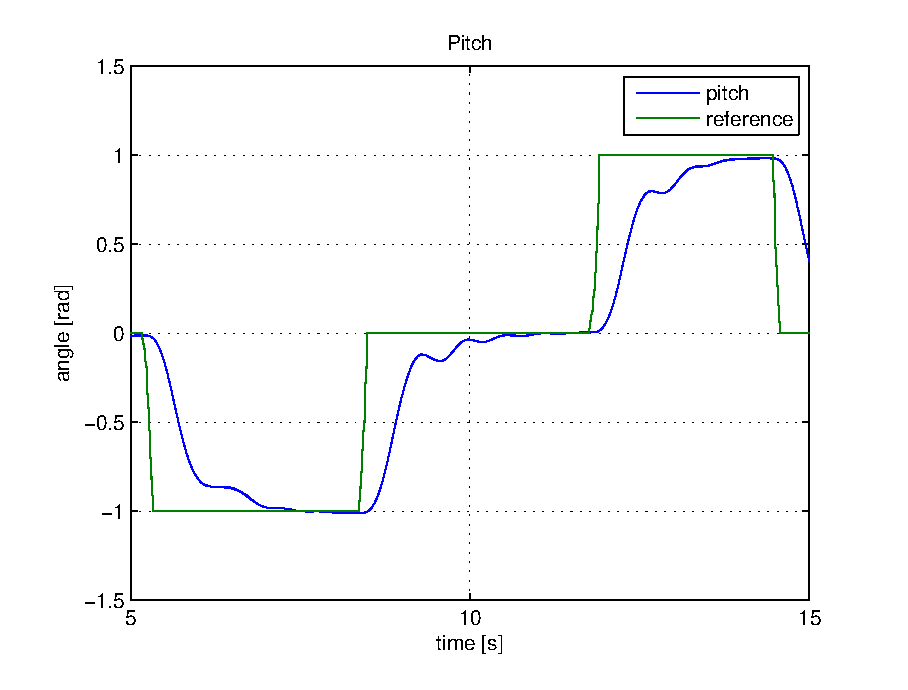
\includegraphics[width=0.9\linewidth]{plots/part2new/pitch_pi.eps}
	    \caption{Pitch with $\omega_0 = \pi$.}
        \label{fig:pitch_pi}
    \end{minipage}%
    \begin{minipage}{.5\textwidth}
        \centering
		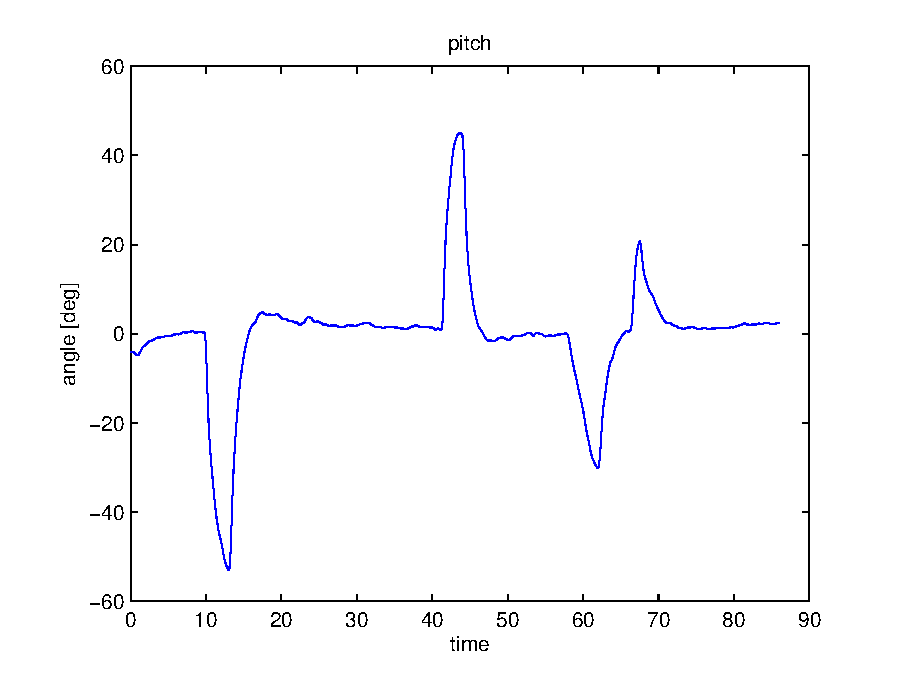
\includegraphics[width=0.9\linewidth]{plots/part2new/pitch_pi_half.eps}
	    \caption{Pitch with $\omega_0 = \pi$/2.}
        \label{fig:pitch_pi_half}
    \end{minipage}%
    \begin{minipage}{.5\textwidth}
    \centering
		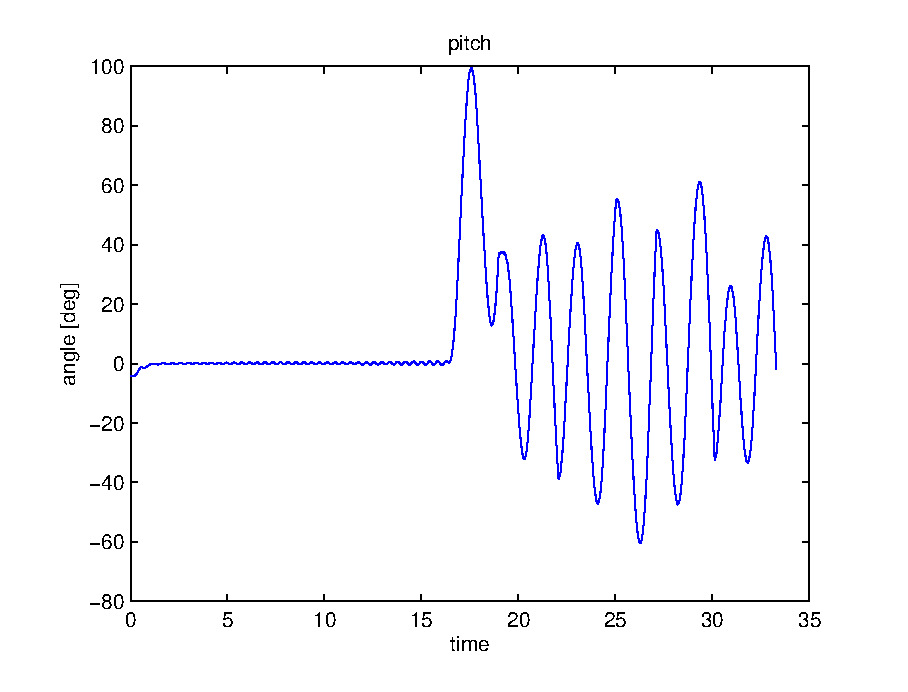
\includegraphics[width=0.9\textwidth]{plots/part2new/pitch_2pi.eps}
	    \caption{Pitch with $\omega_0 = 2 \pi$.}
        \label{fig:pitch_2pi}
    \end{minipage}
    
\end{figure}

%\begin{figure}[htb]
	%\centering
%% 	\hspace{-2.4cm}
%    \begin{minipage}{.5\textwidth}
%	    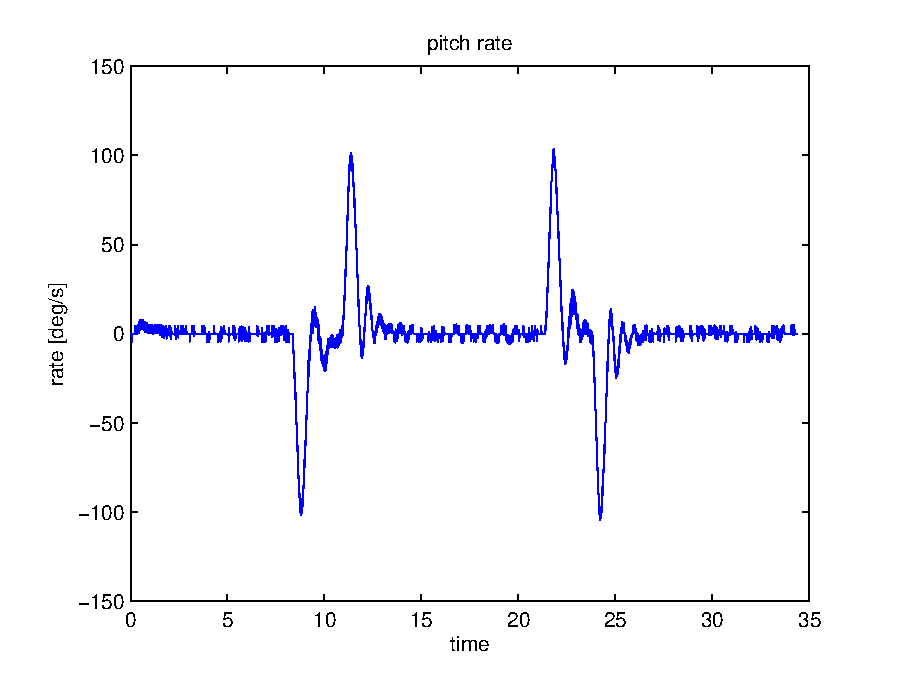
\includegraphics[width=0.9\textwidth]{plots/part2/pitch_rate_pi.eps}
%	    \caption{Pitch rate with $\omega_0 = \pi$.}
%        \label{fig:pitch_rate_pi}
%    \end{minipage}%
%    \begin{minipage}{.5\textwidth}
%        \centering
%		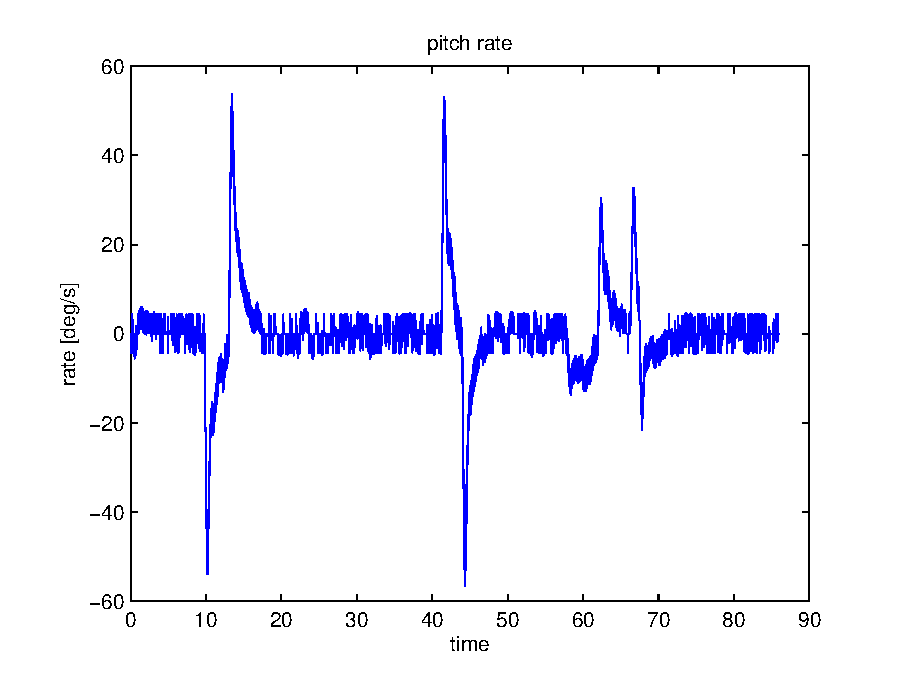
\includegraphics[width=0.9\textwidth]{plots/part2/pitch_rate_pi_half.eps}
%	    \caption{Pitch rate with $\omega_0 = \pi/2$.}
%        \label{fig:pitch_rate_pi_half}
%    \end{minipage}%
%    \begin{minipage}{.5\textwidth}
%    \centering
%		\centering
%		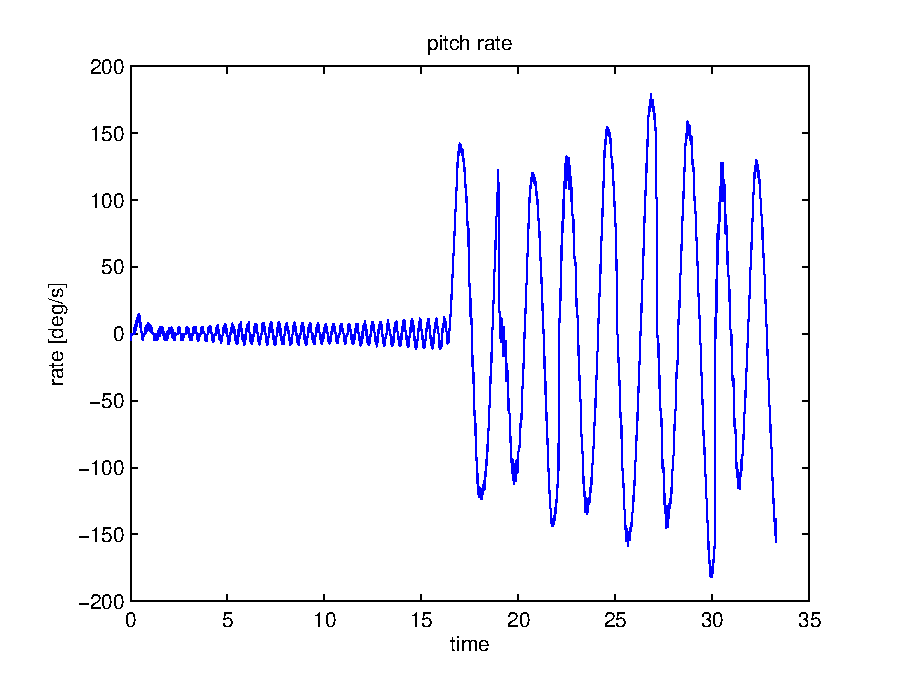
\includegraphics[width=0.9\textwidth]{plots/part2/pitch_rate_2pi.eps}
%	    \caption{Pitch rate with $\omega_0 = 2 \pi$.}
%        \label{fig:pitch_rate_2pi}
%    \end{minipage}
%	
%\end{figure}

As we see, the response is fast an accurate for $\omega_0 = \pi$ in Figures \ref{fig:pitch_pi}. When $\omega_0 = \pi/2$, the pitch angle is slower and does not reach the reference, and as we see from Figure \ref{fig:pitch_pi_half}. $\omega_0 = 2 \pi$ gives unstable oscillations, these would increase if pitch did not have a maximum physical value.
\medskip

By inserting $\omega_0 = \pi$ into eq. (\ref{eq:part2_prob1_K}), we get $K_{pp} = 16.70$ and $K_{pd} = 10.63$.


%%%%%%%%%%%%%%%%%%%%%%%%%%%%%%%%%%%%%%%%%%%%%%%%%%%%%%%%%%%%%%%%%%%%%%%%%%%%%%%%%%%%%%%%%%%%

%%%%                                PART 2 PROBLEM 2

%%%%%%%%%%%%%%%%%%%%%%%%%%%%%%%%%%%%%%%%%%%%%%%%%%%%%%%%%%%%%%%%%%%%%%%%%%%%%%%%%%%%%%%%%%%%
\subsubsection{Problem 2}
We implemented a P controller for travel rate in Simulink as shown in Figure \ref{fig:simulink_travel}.
\begin{figure}[htb]
	\centering
	\includegraphics[trim={0 16cm 16cm 0}, clip,width=\linewidth]{images/simulink/P2_travel.pdf}
	\caption{Simulink diagram for travel rate controller}
    \label{fig:simulink_travel}
\end{figure}

We tuned the controller by trying different values of $K_{rp}$ until we found a satisfying response. The plots in Figures \ref{fig:travel_1_1}-\ref{fig:travel_1_5} shows two different choices of $K_{rp}$.
\begin{figure}[htb]
	%\centering
	\hspace{-2.7cm}
	\begin{minipage}{.5\textwidth}
	    \centering
		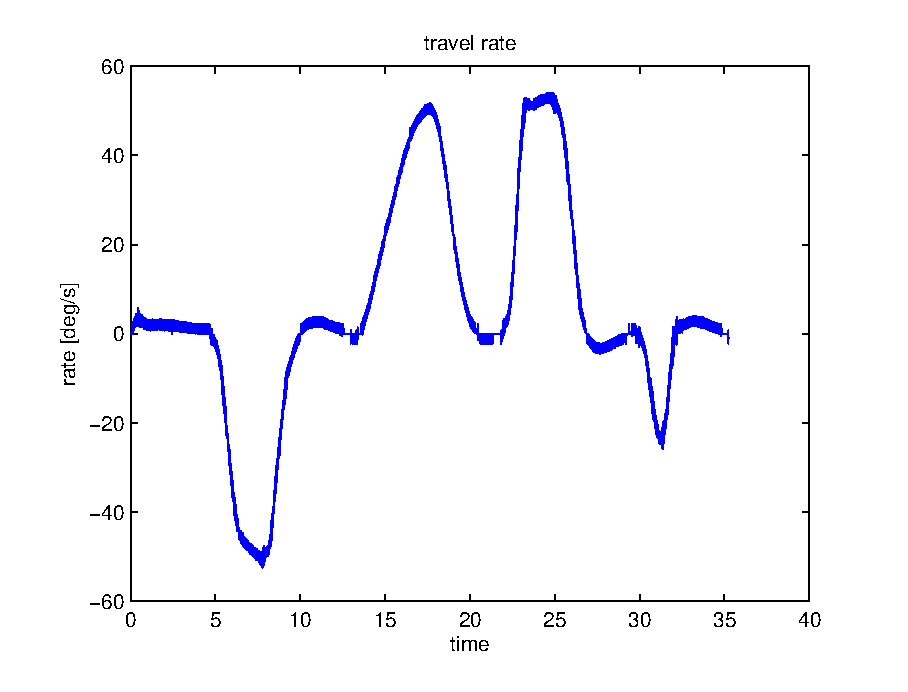
\includegraphics[width=0.9\linewidth]{plots/part2new/travel_rate_1_1.eps}
	    \caption{Travel rate, $K_{rp} = -1.1$.}
        \label{fig:travel_1_1}
    \end{minipage}%
    \begin{minipage}{.5\textwidth}
        \centering
		\includegraphics[width=0.9\linewidth]{plots/part2new/travel_rate_0_5.eps}
	    \caption{Travel rate, $K_{rp} = -0.5$.}
        \label{fig:travel_half}
    \end{minipage}%
    \begin{minipage}{.5\textwidth} 
    \centering 
		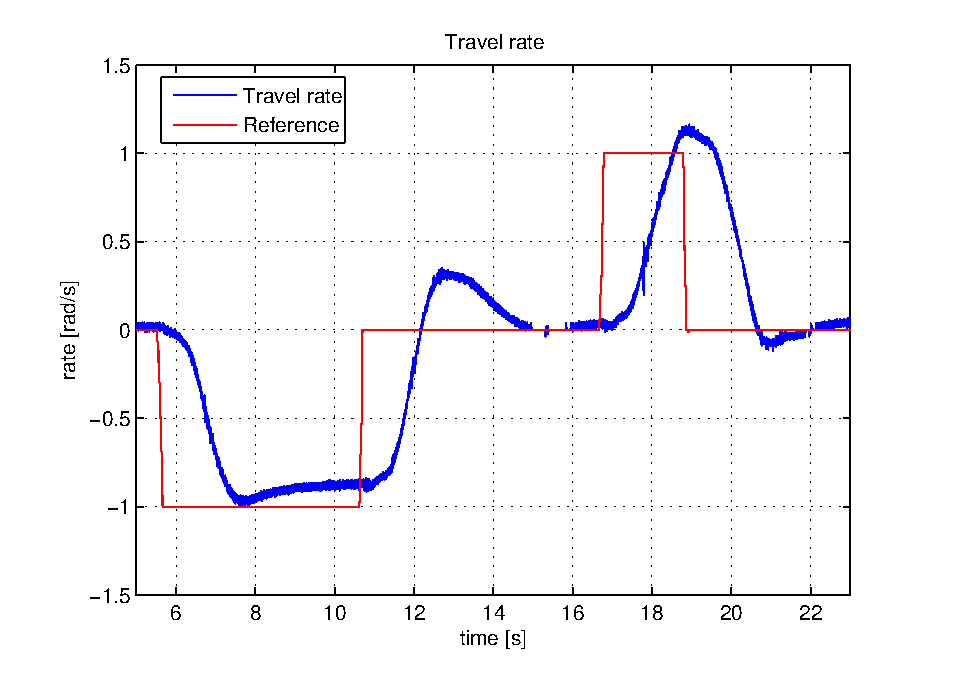
\includegraphics[width=0.9\textwidth]{plots/part2new/travel_rate_1_5.eps}
	    \caption{Travel rate, $K_{rp} = -1.5$.}
        \label{fig:travel_1_5}
    \end{minipage}
    
\end{figure}
Choosing $K_{rp} = -1.1$ gave the faster and more accurate response.


\subsection{Part 3}
\subsubsection{Problem 2}
%%%%%%%%%%%%%%%%%%%%%%%%%%%%%%%%%%%%%%%%%%%%%%%%%%%%%%%%%%%%%%%%%%%%%%%%%%%%%%%%%%%%%%%%%%%%

%%%%                                PART 3 PROBLEM 2

%%%%%%%%%%%%%%%%%%%%%%%%%%%%%%%%%%%%%%%%%%%%%%%%%%%%%%%%%%%%%%%%%%%%%%%%%%%%%%%%%%%%%%%%%%%%

We now add an LQR controller to our system, aiming to control the pitch angle and elevation rate. The controller is given by eq. (\ref{eq:part3_prob2_state_feedback}). The Simulink diagram can be seen in Figure \ref{fig:simulink_multivariabe}.\medskip

\begin{figure}[h!]
	\centering
	\includegraphics[scale=0.8, trim={0 12cm 16cm 0}, clip]{images/simulink/P3.pdf}
	\caption{Simulink diagram for multivariable controller}
    \label{fig:simulink_multivariabe}
\end{figure}


When tuning the weighting matrices \textbf{Q} and \textbf{R} we have to  keep the system as close to the linearized model as possible or the assumptions made in (\ref{eq:state_space}) will no longer be valid. We started with $1$ on all the values. We want to control pitch and elevation rate, so these values were increased if the system was to slow/far away from the references. When the system would overshoot, we increased the value in $R$, so that the regulator can't use as much input, and lowered them when they failed to reach the reference. After repeating these steps a few times we found our final values. The final weighting matrices are seen in (\ref{eq:Q_p}) and (\ref{eq:R_p}). 

\begin{equation} \label{eq:Q_p}
    \bm{Q} = 
	\begin{bmatrix}
		10000 & 0     & 0\\
		0     & 10    & 0\\
		0     & 0     & 100000\\
	\end{bmatrix}
\end{equation} 

\begin{equation} \label{eq:R_p}
    \bm{R} = 
	\begin{bmatrix}
		100   & 0  \\
		0     & 100\\
	\end{bmatrix}
\end{equation} 

With these weighting matrices, $\bm{K}$ and $\bm{P}$ become
\begin{equation} \label{eq:K_p}
    \bm{K} = 
	\begin{bmatrix}
		0     & 0     & 31.62\\
		10    & 5.828 & 0    \\
	\end{bmatrix}
\end{equation} 

\begin{equation} \label{eq:P_p}
    \bm{P} = 
	\begin{bmatrix}
		0     & 31.62\\
		10    & 0    \\
	\end{bmatrix}
\end{equation} 

The resulting responses for elevation rate and pitch angle can be seen in Figure \ref{fig:Elevationrate_p} and \ref{fig:Pitch_p}.

\begin{figure}[h!]
	%\centering
 	%\hspace{-2.4cm}
    \begin{minipage}{.45\textwidth}
	    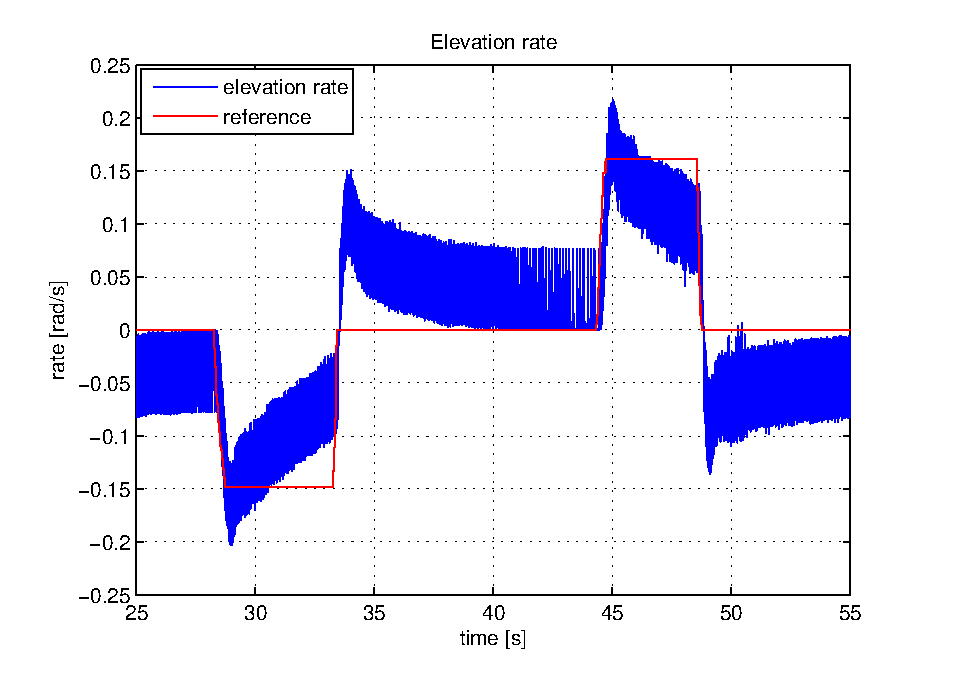
\includegraphics[width=1\textwidth]{plots/part3/part2/Elevationrate.eps}
	    \caption{Elevation rate with LQR.}
        \label{fig:Elevationrate_p}
    \end{minipage}\hspace{0.1\textwidth}%
    \begin{minipage}{.45\textwidth}
        \centering
		\includegraphics[width=1\textwidth]{plots/part3/part2/Pitch.eps}
	    \caption{Pitch with LQR.}
        \label{fig:Pitch_p}
    \end{minipage}
\end{figure}
\medskip

From Figure \ref{fig:Elevationrate_p} we can see that the LQR controller alone is not enough to control the elevation rate. This is a result of having a linearized model. As the helicopter moves away from the zero state the nonlinearity in (\ref{eq:model_se_al_elev}) forces the helicopter back to its zero state. 

%%%%%%%%%%%%%%%%%%%%%%%%%%%%%%%%%%%%%%%%%%%%%%%%%%%%%%%%%%%%%%%%%%%%%%%%%%%%%%%%%%%%%%%%%%%%

%%%%                                PART 3 PROBLEM 3

%%%%%%%%%%%%%%%%%%%%%%%%%%%%%%%%%%%%%%%%%%%%%%%%%%%%%%%%%%%%%%%%%%%%%%%%%%%%%%%%%%%%%%%%%%%%
\subsubsection{Problem 3}
We wanted to include the integral effect to mitigate the effects of linearizing the model, this is most significant for $\dot{\tilde{e}}$. This works by integrating the steady state error that occurs from the change of gravitational force on the helicopter when it moves away from the zero state. In effect this will set a reference elevation that the the system til try to return to, even when exposed to external physical disturbances. 
\medskip

The Simulink model for the multivariable controller with integral effect can be seen in Figure \ref{fig:simulink_multivariable_integral}.

\begin{figure}[h]
	\centering
	\includegraphics[trim={0 7cm 12cm 0}, clip,scale=0.6]{images/simulink/P3_integral.pdf}
	\caption{Simulink diagram for multivariable controller with integral effect.}
    \label{fig:simulink_multivariable_integral}
\end{figure}

\medskip

When deciding how to weight $\dot{\gamma}$ and $\dot{\zeta}$ we knew that the pitch using the LQR controller already gave us good results, while the elevation rate would be more dependant on the integral effect. We therefore weighted $\dot{\gamma}$ lower than $\dot{\zeta}$ which we weigh quite high. After tuning the controller the final values for $\bm{Q}_i$ and $\bm{R}_i$ are

\begin{equation} \label{eq:Q_pi}
    \bm{Q}_i = 
	\begin{bmatrix}
		10000 &  0    &  0      &  0   &  0 \\
		0     &  10   &  0      &  0   &  0 \\
		0     &  0    &  10000  &  0   &  0 \\
		0     &  0    &  0      &  100 &  0 \\
		0     &  0    &  0      &  0   &  10000
	\end{bmatrix}
\end{equation} 

\begin{equation} \label{eq:R_pi}
    \bm{R}_i = 
	\begin{bmatrix}
		75   & 0  \\
		0    & 100\\

	\end{bmatrix}
\end{equation} 

After optimizing the cost function (\ref{eq:cost_function}) using the matlab command \texttt{lqr(A, B, Q, R)} - where \texttt{A}, \texttt{B}, \texttt{Q} and \texttt{R} are  respectively $\bm{A}_i$, $\bm{B}_i$, $\bm{Q}_i$ and $\bm{R}_i$,
we acquire the following $\bm{K}_i$ matrix

\begin{equation} \label{eq:K_pi}
    \bm{K}_i = 
	\begin{bmatrix}
		0      &  0      & 17.62 &  0     &  10 \\
		12.04  &  7.13   & 0     &  3.16  &  0 \\
	\end{bmatrix}
\end{equation} 

The resulting response can be seen in Figure \ref{fig:Elevationrate_pi} and \ref{fig:Pitch_p_integral}.
\begin{figure}[h!]
	%\centering
 	%\hspace{-2.4cm}
    \begin{minipage}{.45\textwidth}
	    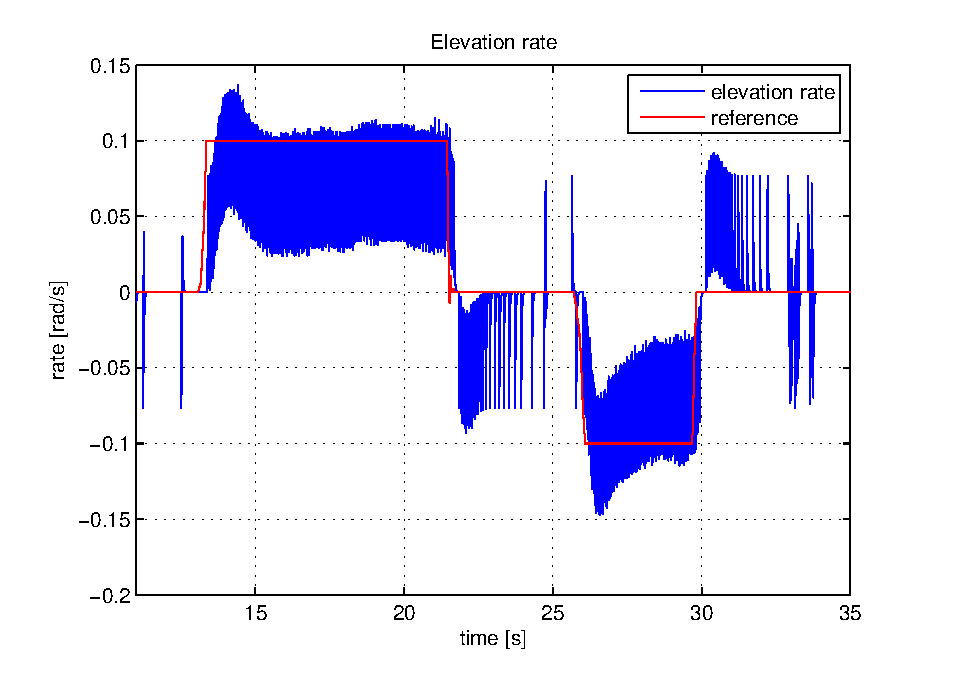
\includegraphics[width=1\textwidth]{plots/part3/part3_integral/elevationrate.eps}
	    \caption{Elevation rate with LQR and integral effect.}
        \label{fig:Elevationrate_pi}
    \end{minipage}\hspace{0.1\textwidth}%
    \begin{minipage}{.45\textwidth}
        \centering
		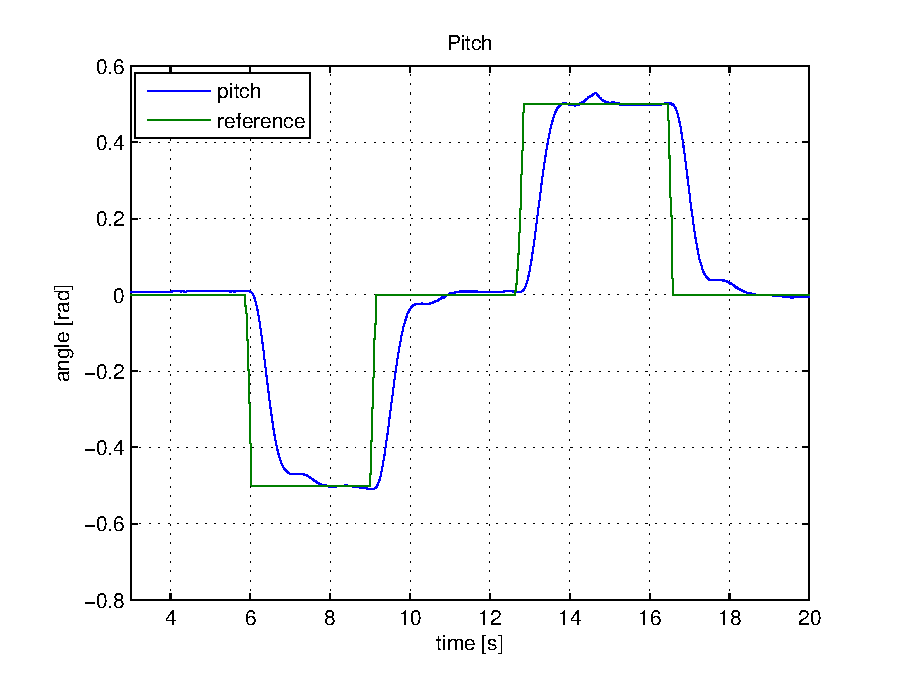
\includegraphics[width=1\textwidth]{plots/part3/part3_integral/pitch.eps}
	    \caption{Pitch with LQR and integral effect.}
        \label{fig:Pitch_p_integral}
    \end{minipage}
\end{figure}
As we see, the elevation rate does not go back to zero as it did with just the LQR in Figure \ref{fig:Elevationrate_p}. The pitch angle in Figure \ref{fig:Pitch_p_integral} is still fast and accurate, the response is about the same as we saw with LQR in Figure \ref{fig:Pitch_p}.

\subsection{Part 4}
%%%%%%%%%%%%%%%%%%%%%%%%%%%%%%%%%%%%%%%%%%%%%%%%%%%%%%%%%%%%%%%%%%%%%%%%%%%%%%%%%%%%%%%%%%%%

%%%%                                PART 4 PROBLEM 1

%%%%%%%%%%%%%%%%%%%%%%%%%%%%%%%%%%%%%%%%%%%%%%%%%%%%%%%%%%%%%%%%%%%%%%%%%%%%%%%%%%%%%%%%%%%%
\subsubsection{Problem 1}
Implemented our new model in Simulink. 
\begin{figure}[h!]
    \centering
	\includegraphics[trim={0 3cm 0 3cm},clip,width=\linewidth]{images/simulink/P4_diag.pdf}
    \caption{Simulink model with observer subsystem}
    \label{fig:simulink_P4}
\end{figure}

\begin{figure}[H]
    \centering
	\includegraphics[trim={6.5cm 6.5cm 6.5cm 6.5cm},clip,width=\linewidth]{images/simulink/P4_observer.pdf}
    \caption{Simulink model of observer}
    \label{fig:simulink_P4_observer}
\end{figure}

The estimator is used as input to the controller, instead of the actual measurements $y$. To calculate the estimator, the matrices from the linearized system have been used. This means that the estimator, just like our modelled system, works best when close to the equilibrium. When the system moved away from this point, both the system and the estimator will differ from the real world, meaning that the regulator won't be able to fully regulate the system to the reference. 

%%%%%%%%%%%%%%%%%%%%%%%%%%%%%%%%%%%%%%%%%%%%%%%%%%%%%%%%%%%%%%%%%%%%%%%%%%%%%%%%%%%%%%%%%%%%

%%%%                                PART 4 PROBLEM 2

%%%%%%%%%%%%%%%%%%%%%%%%%%%%%%%%%%%%%%%%%%%%%%%%%%%%%%%%%%%%%%%%%%%%%%%%%%%%%%%%%%%%%%%%%%%%
\subsubsection{Problem 2}
The estimator poles need to be placed in such a way that the estimator will be able to predict the error faster than the system. This means putting the estimator poles further out into the left plane. We used \texttt{r = 10*max(abs(eig(A-BK)))} which gave us an $r = 24$ as a base for our tuning, and adjusted the r value until the estimator followed the actual system without a lot of noice. Matlab code for computing the poles can be found in appendix \ref{sec:matlab_pole_placement}. Some example responses for different values of r can be seen in Figures \ref{fig:e_rate_5}, \ref{fig:e_rate_27} and \ref{fig:e_rate_60}.\\

\begin{figure}[H]
	%\centering
	\hspace{-2.7cm}
	\begin{minipage}{.5\textwidth}
	    \centering
		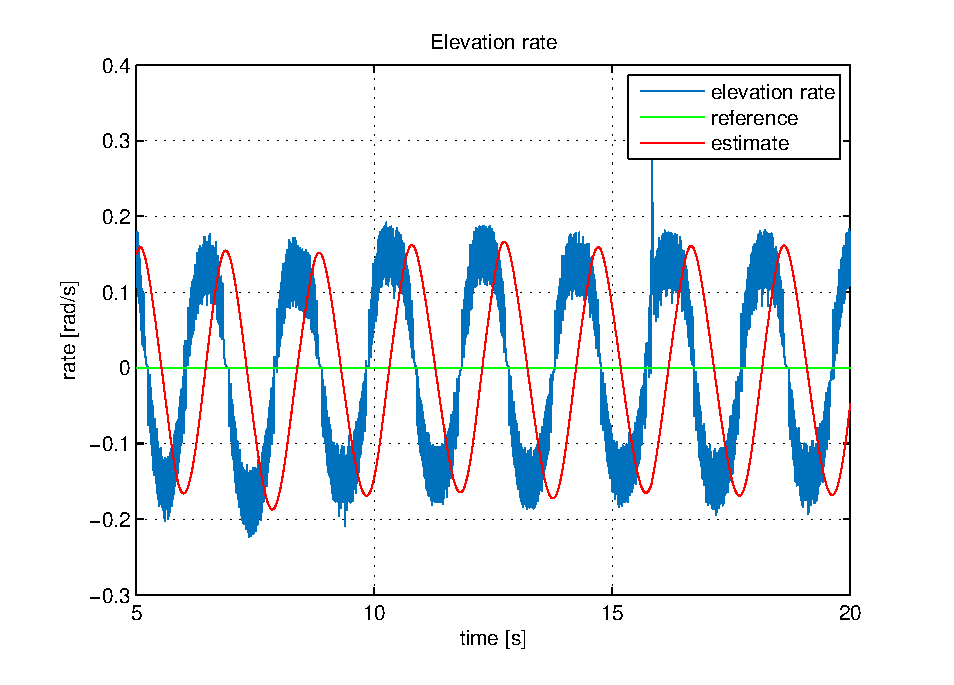
\includegraphics[width=0.9\linewidth]{plots/part4new/P/e_rate_5.eps}
	    \caption{Elevation rate with r = 5.}
        \label{fig:e_rate_5}
    \end{minipage}%
    \begin{minipage}{.5\textwidth}
        \centering
		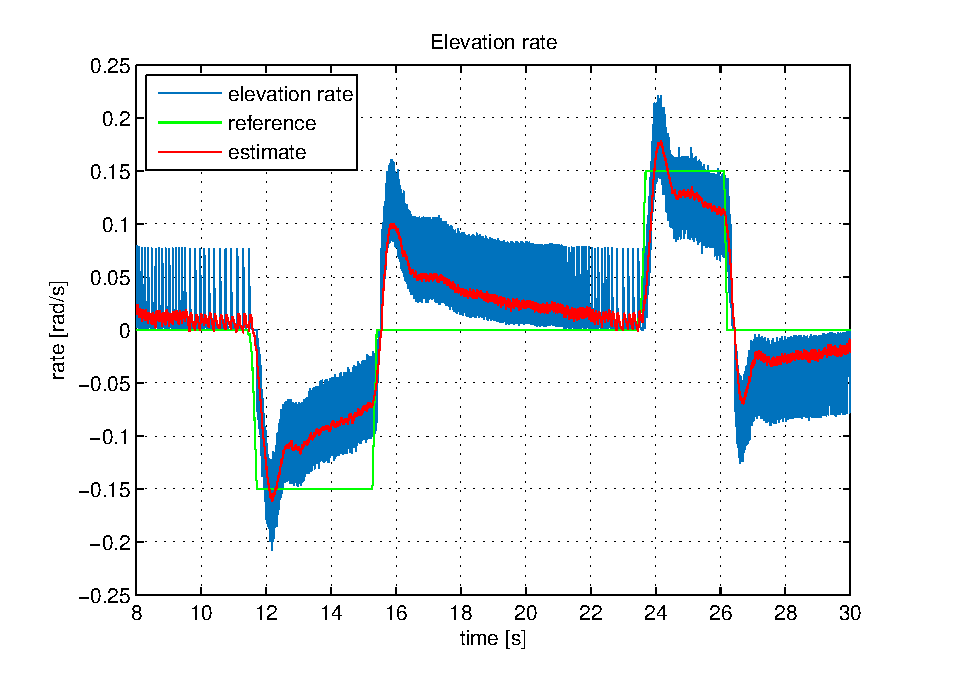
\includegraphics[width=0.9\linewidth]{plots/part4new/P/e_rate_27.eps}
	    \caption{Elevation rate with r = 27.}
        \label{fig:e_rate_27}
    \end{minipage}%
    \begin{minipage}{.5\textwidth}
    \centering
		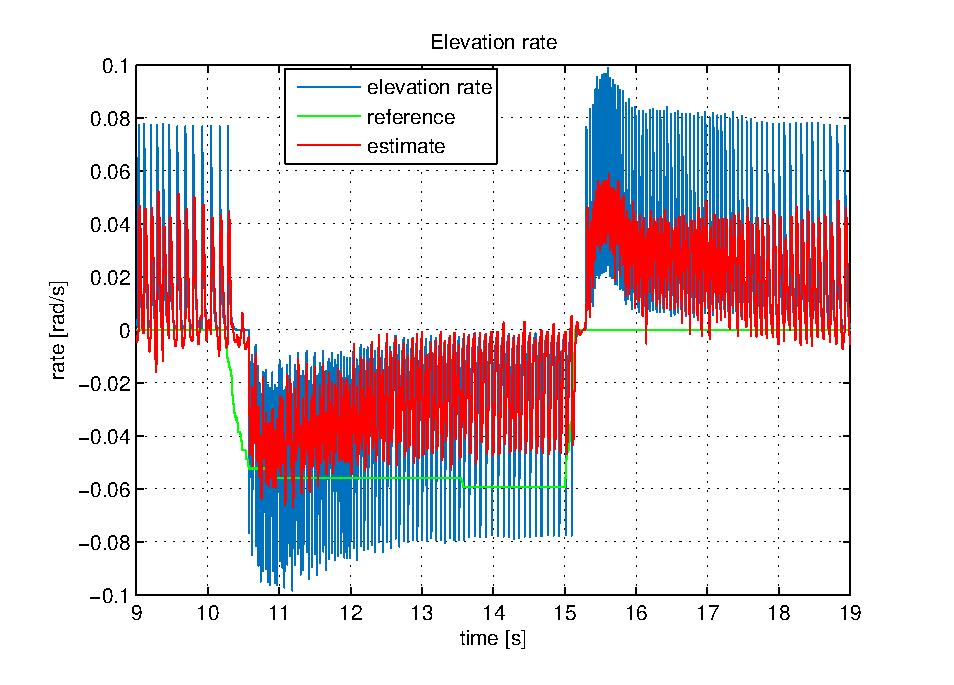
\includegraphics[width=0.9\textwidth]{plots/part4new/P/elevation_rate_60.eps}
	    \caption{Elevation rate with r = 60.}
        \label{fig:e_rate_60}
    \end{minipage}
\end{figure}

These three figures demonstrate what happens when the poles are placed either too close to the origin, just right, and too far away. \Cref{fig:e_rate_5} has the poles at $r=5$. This is not big enough for the estimator to predict the system fast enough. As we see on the plot it creates a phase lag, and this results in the system not staying at the reference, which is $0$. Our controller attempts to use the estimator to keep the system at the reference, when the estimator is too slow, the prediction will already have happened, meaning the controller is always reacting to late.\medskip

\Cref{fig:e_rate_60} shows the opposite behaviour, with poles with a too large radius. This plot shows the behaviour for $r=60$. Now the estimator is fast enough to predict the system. But where the small radius has a strong low filtering property, we see that this estimator doesn't. This causes a lot of noise on the estimator. A noisy estimator doesn't contribute anything useful to the system, and we didn't notice any big difference in the helicopter behaviour compared to the system without an estimator. Comparing the plots in \cref{fig:Elevationrate_pi} and the blue line in \cref{fig:e_rate_60}, also shows this behaviour.\medskip

The figure in the middles, \cref{fig:e_rate_27} show our final result. Here the poles are placed as shown in \cref{fig:pole_placement}, with a radius $r=27$. The estimator is fast enough to now predict the system, while still suppressing the noise from the elevation rate measurements by using its low pass characteristics.\medskip

\begin{figure}[H]
    \centering
	\includegraphics[width=0.9\linewidth]{plots/part4new/P/poles.eps}
    \caption{Pole placement for P controller. System poles:\textbf{\textcolor{red}{+}}, estimator poles:\textcolor{blue}{o}}

    \label{fig:pole_placement}
\end{figure}

We can further improve the system by implementing an integral effect as we did in part 3 problem 3. We found we got better results here by increasing the radius of the poles slightly and the final result of this can be seen in Figure \ref{fig:e_rate_42}.\\\medskip

\begin{figure}[H]
    \centering
	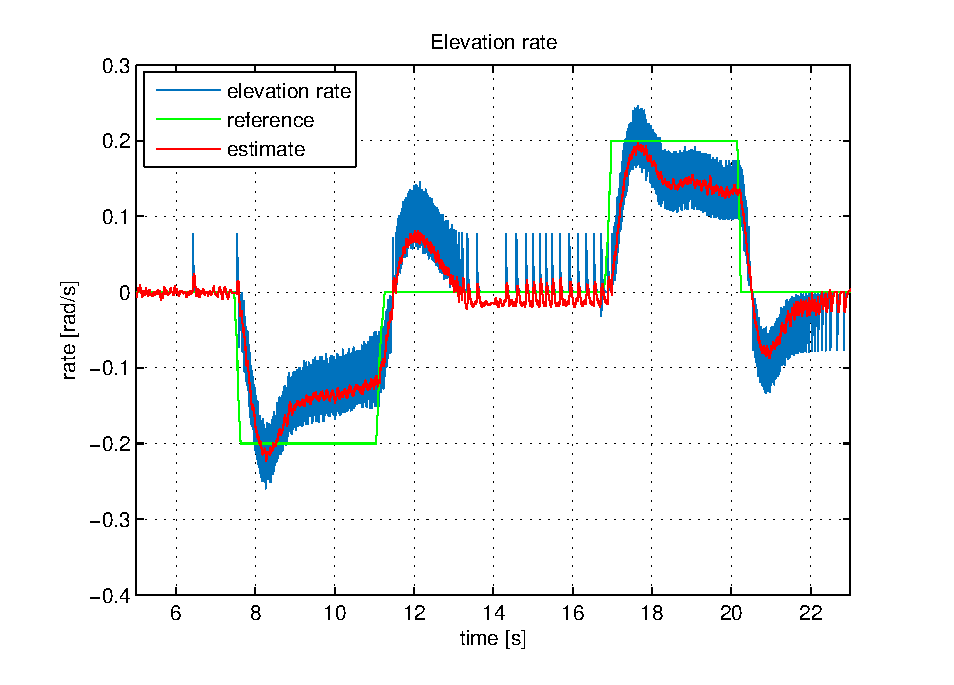
\includegraphics[width=0.9\linewidth]{plots/part4new/PI/e_rate_42.eps}
    \caption{Elevation rate with r = 42 and controller with integral effect}

    \label{fig:e_rate_42}
\end{figure}

%%%%%%%%%%%%%%%%%%%%%%%%%%%%%%%%%%%%%%%%%%%%%%%%%%%%%%%%%%%%%%%%%%%%%%%%%%%%%%%%%%%%%%%%%%%%

%%%%                                PART 4 PROBLEM 3

%%%%%%%%%%%%%%%%%%%%%%%%%%%%%%%%%%%%%%%%%%%%%%%%%%%%%%%%%%%%%%%%%%%%%%%%%%%%%%%%%%%%%%%%%%%%
\subsubsection{Problem 3}


In the final part of the lab assignment, our goal was to see whether we could use an estimator to control the system if we changed $y$. As shown in \cref{sec:P4p3}, only measuring pitch and elevation meant the system wouldn't be observable. However, by only measuring the elevation and travel, the system could be observed. This is because of the connection between travel and pitch, given by \cref{eq:model_linearized_lambda}. This allows the estimator to predict what the pitch is based on its knowledge of $\lambda$. \medskip

Even though the system is observable, it is harder to tune the controller. If the controller is to predict the pitch, it will need to differentiate the travel measurement, twice. It is a bad idea to differentiate a signal because differentiating noise creates even more, stronger noise. So differentiating noise twice isn't a good thing either.\medskip

\begin{figure}[H]
    \centering
	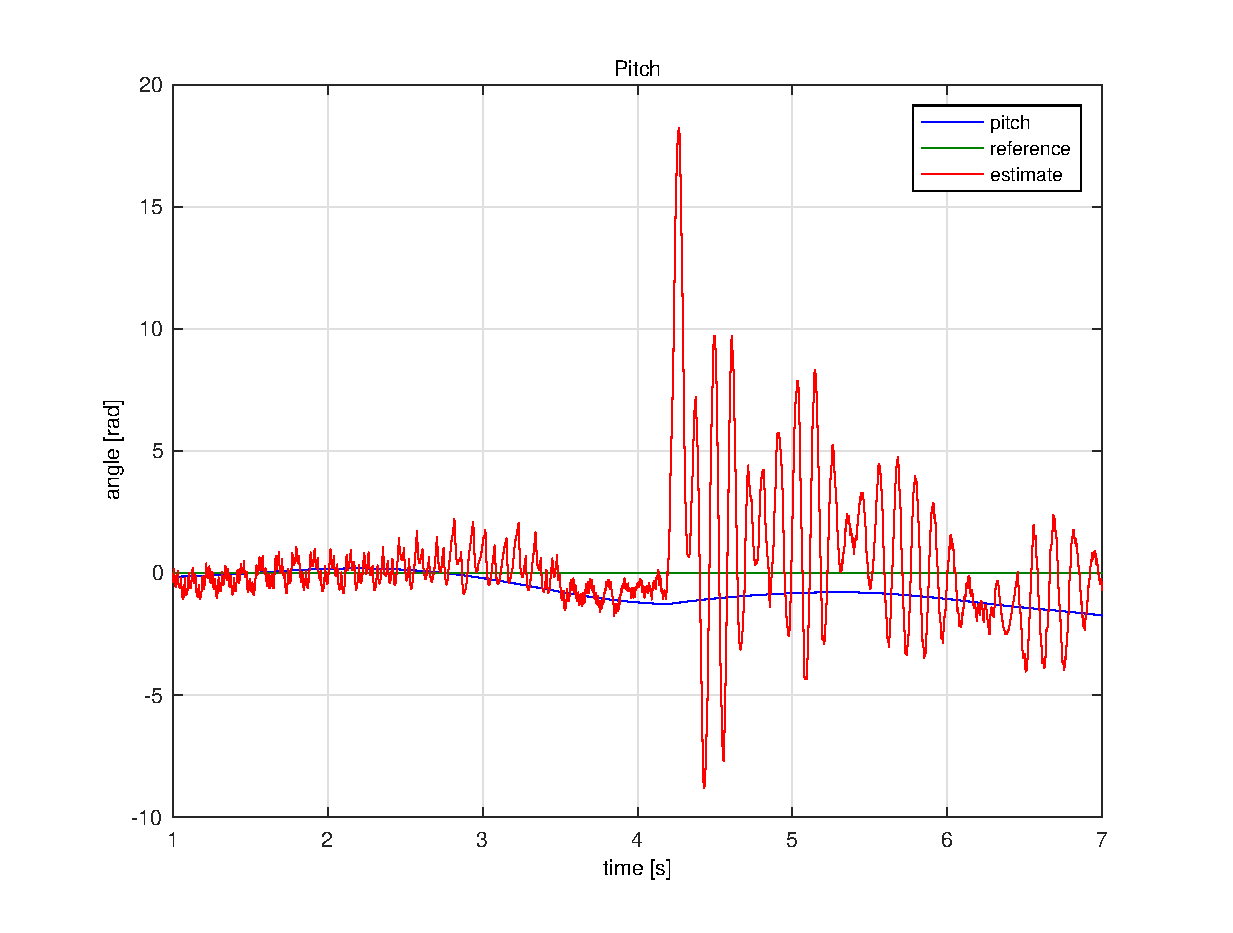
\includegraphics[width=0.9\linewidth]{plots/part4new/pitch_bad.eps}
    \caption{Pitch when pitch and elevation is measured.}
    \label{fig:BAD}
\end{figure}

\Cref{fig:BAD} shows this behaviour. The estimator thinks that the helicopter is swinging a lot around the $p$ joint, while it in reality is just leaning to one side. The controller uses the estimated value for control, and because of this, the system is hard to tune for pitch. The elevation is passed into the observer block, and is therefor easier to control.

When deciding how to tune the system we had to reduce the weight of the integrating factors dramatically as these produced an uncontrollable amount of noise, but we could not remove the entirely as steady state errors are expected when only being able to observe the travel to calculate the pitch. We also reduced the rest of the values in the system overall. The system is therefore slower, but when regulating a signal with a high amount of noise it is favorable that the system is ``sure'' of a change in pitch before responding. As the elevation estimated quite well the cost of regulating it is cheaper than regulating the pitch. The final \textbf{Q} and \textbf{R} can be seen in equations


\begin{equation} \label{eq:Q_P4p3}
    \bm{Q}_i = 
	\begin{bmatrix}
		150 &  0    &  0      &  0   &  0 \\
		0     &  10   &  0      &  0   &  0 \\
		0     &  0    &  150  &  0   &  0 \\
		0     &  0    &  0      &  10 &  0 \\
		0     &  0    &  0      &  0   &  10
	\end{bmatrix}
\end{equation} 

\begin{equation} \label{eq:R_P4p3}
    \bm{R}_i = 
	\begin{bmatrix}
		2   & 0  \\
		0    & 20\\

	\end{bmatrix}
\end{equation} 

The pole placement of the observer is also of paramount importance, and the system was highly sensitive to their placement. Poles at to close of a radius caused exponential oscillations, the observer is to slow to react to changes and the propellers simply vibrate at a high frequency. If the poles are to far away the integral effect causes the pitch and elevation to increase exponentially in one direction as the system is to slow to react to the estimated changes and the integral effect dominates. While tuning we found we got better responses by placing all poles close to each other on the real axis and settled on having the closest pole at -25.928\footnote{the system was so sensitive that three decimal places were necessary} and the other poles at 0.1 increments behind. The poles can be seen in Figure \ref{fig:P4p3_poles}.

\begin{figure}[H]
    \centering
	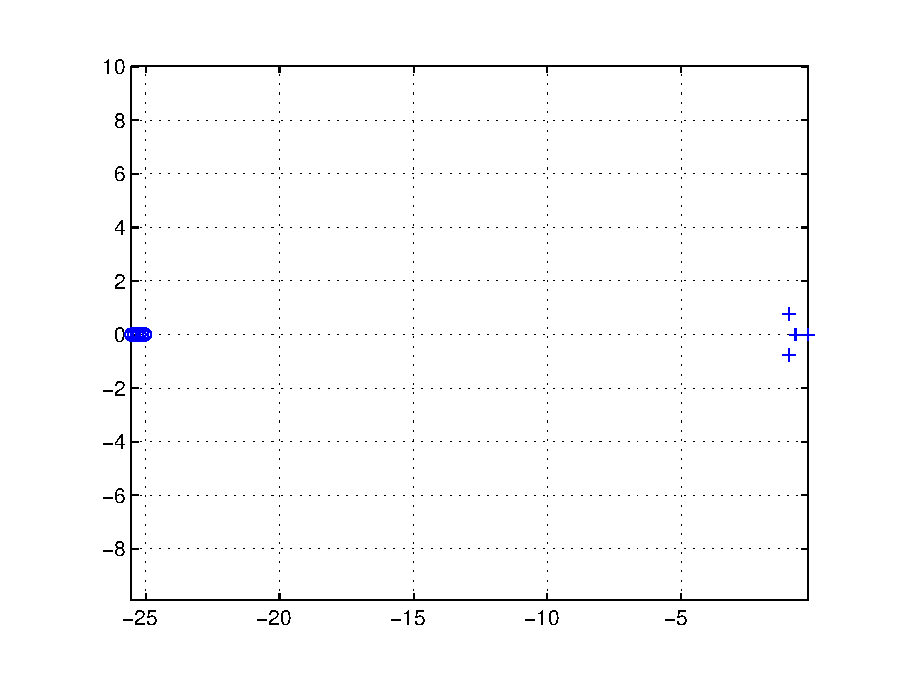
\includegraphics[width=0.9\linewidth]{plots/part4new/P4p3_poles.eps}
    \caption{Poles of the stable observer system}
    \label{fig:P4p3_poles}
\end{figure}

The final response of the system can be seen in Figure \ref{fig:P4p3_pitch}. 

\begin{figure}[H]
    \centering
	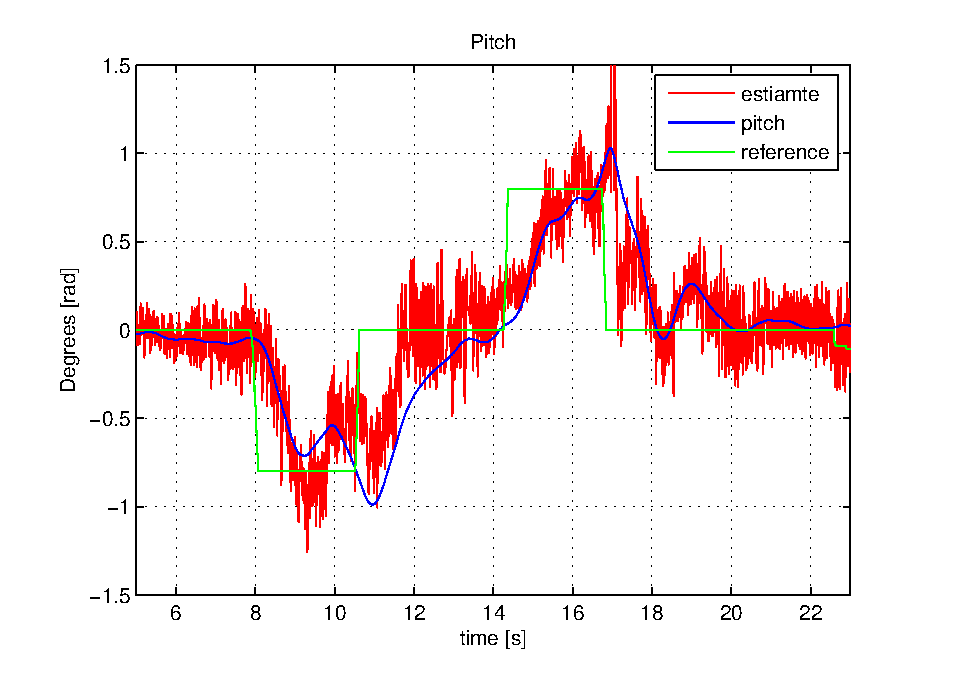
\includegraphics[width=0.9\linewidth]{plots/part4new/P4p3_bra_pitch.eps}
    \caption{Pitch of the system using the bad observer}
    \label{fig:P4p3_pitch}
\end{figure}

In conclusion; just because a system is observable for certain values it will not necessarily result in a well regulated system, it may be a good idea to apply a PBH test\footnote{Popov-Belevitch-Hautus test. Used to determine how controllable or observable a system is.} when one only has access to a limited number of states \cite{youtube}.

\newpage

\section{Conclusions}
In this assignment we have tried different controllers on the same system. The system works best around the equilibrium, which is as expected as the linear model simplifies the system, and ignores the effect caused by the pitch and elevation angles.\medskip

In the first part, the system was controlled using feed-forward. This didn't work well. The second task uses monovariable controllers, which work fine. The downside here is that we need a separate controller for each state. This means a lot of tuning, and work.\medskip

The multivariable controllers, using LQR, controlled all states with one common controller. This meant that tuning was easier, and the results better. We did however need two additional states, the integral effects, for it to work best. We used these two controllers together with an estimator. The estimator poles had to be placed in the correct area. When placed here, it could estimate the system while providing a low pass filtered signal for our controllers. This improved the system behaviour. The estimator requires the system to be observable, but as we saw in the last section, this doesn't guarantee a system that can be nicely controlled. Differentiating a measurement gives a lot of noise, and we tried to differentiate our measurement twice in our estimator. Therefor the last part was hard to control. 

\clearpage
\appendix\section{Nomenclature}\label{sec:nomenclature}


%% CONSTANTS
\begin{table}[h!]
	\centering
	\caption{Parameters and values.}
	\begin{tabular}{llll}
		\toprule
		Symbol & Parameter & Value & Unit \\
		\midrule
	    $e^\ast$    & Linearization point, elevation angle            & $0$     & \rad                        \\
		$F_{g,b}$   & Gravitational force, back motor                 & $7.063$ & \newton                     \\
		$F_{g,c}$   & Gravitational force, counterweight              & $18.84$ & \newton                     \\
		$F_{g,f}$   & Gravitational force, front motor                & $7.063$ & \newton                     \\
		$g$         & Gravitational acceleration                      & $9.81$  & \meter\per\second\squared   \\
		$J_e$       & Moment of inertia for elevation                 & $1.036$ & \kilogram\usk\meter\squared \\
		$J_\lambda$ & Moment of inertia for travel                    & $1.078$ & \kilogram\usk\meter\squared \\
		$J_p$       & Moment of inertia for pitch                     & $0.044$ & \kilogram\usk\meter\squared \\
		$K_f$       & Motor force constant                            & $0.149$ & \newton\per\volt            \\
		$l_{c}$     & Distance from elevation axis to counterweight   & $0.46$  & \meter                      \\
		$l_{h}$     & Distance from elevation axis to helicopter head & $0.66$  & \meter                      \\
		$l_{p}$     & Distance from pitch axis to motor               & $0.175$ & \meter                      \\
%		$m_h$       & Mass of helicopter                              & $1.05$  & \kilogram                   \\
		$m_{p}$     & Motor mass                                      & $0.72$  & \kilogram                   \\
  		$m_{c}$     & Counterweight mass                              & $1.92$  & \kilogram                   \\
  		$p^\ast$    & Linearization point, pitch angle                & $0$     & \rad                        \\
  		$V_d^\ast$  & Linearization point, voltage difference         & $0$     & \volt                       \\
  		$V_s^\ast$  & Linearization point, voltage sum                & $6.711$ & \volt                       \\
  		$\lambda^\ast$    & Linearization point, travel angle         & $0$     & \rad                        \\
		\bottomrule
	\end{tabular}
\label{tab:constans}
\end{table}

%% VARIABLES AND OTHER PARAMETERS

\begin{table}[h!]
	\centering
	\caption{Parameters and values.}
	\begin{tabular}{lll}
		\toprule
		Symbol & Parameter & Unit \\
		\midrule
		$e$         & Elevation angle                                   & \rad                        \\
		$\tilde{e}$ & Elevation angle, after coordination transform     & \rad                        \\
		$\tilde{e}_c$ & Elevation angle reference                       & \rad                        \\
		$F_b$       & Force from back propeller                         & \newton                     \\
		$F_f$       & Force from front propeller                        & \newton                     \\
		$J$         & Moment of inertia                                 & \kilogram\meter\squared     \\
		$\bm{J}$    & Cost function for linear quadratic regulator      & $-$                         \\
		$K_{pd}$    & Controller gain                                   & $-$                         \\
		$K_{pp}$    & Controller gain                                   & $-$                         \\
		$K_{rd}$    & Controller gain                                   & $-$                         \\
		$\bm{K}$    & Gain matrix for linear quadratic regulator        & $-$                         \\
		$\bm{L}$    & Gain matrix for linear observer                   & $-$                         \\
		$M$         & Torque                                            & \newton\meter               \\
		$p$         & Pitch angle                                       & \rad                        \\
		$\tilde{p}$ & Pitch angle, after coordination transform         & \rad                        \\
		$\tilde{p}_c$ & Pitch angle reference                           & \rad                        \\
		$\bm{P}$    & Gain matrix                                       & $-$                         \\
		$\bm{Q}$    & Weighting matrix for linear quadratic regulator   & $-$                         \\
		$\bm{r}$    & Reference vector                                  & $-$                         \\
		$\bm{R}$    & Weighting matrix for linear quadratic regulator   & $-$                         \\
		$t$         & Time                                              & \second                     \\
		$\bm{u}$    & Input vector                                      & $-$                         \\
		$V_b$       & Voltage back motor                                & \volt                       \\
		$V_d$       & Voltage difference                                & \volt                       \\
		$\tilde{V}_d$     & Voltage difference, after coordinate transform  & \volt                       \\
		$V_f$       & Voltage front motor                               & \volt                       \\
		$V_s$       & Voltage sum                                       & \volt                       \\
		$\tilde{V}_s$     & Voltage sum, after coordinate transform     & \volt                       \\
		$\bm{x}$    & State vector                                      & $-$                         \\
		$\bm{y}$    & Output vector                                     & $-$                         \\
  		$\lambda$         & Travel angle                                & \rad                        \\
		$\tilde{\lambda}$ & Travel angle, after coordination transform  & \rad                        \\
		$\dot{\tilde{\lambda}}_c$ & Elevation rate reference            & \rad\per\second             \\
		
		\bottomrule
	\end{tabular}
\label{tab:parameters}
\end{table}


\clearpage
    \section{Matlab code snippets}\label{sec:matlab_snippets}
\subsection{Pole placement} \label{sec:matlab_pole_placement}
\lstinputlisting{code/Pole_placement_short.m}

\bigskip

\subsection{Observability} \label{sec:matlab_observability}
\lstinputlisting{code/Observability_short.m}





% References
\newpage
\addcontentsline{toc}{section}{References}
\printbibliography{}
\label{sec:bibliography}
\end{document}
